\chapter{Simulations}
This chapter presents the results obtained by simulations. The research has been made for two models
described in chapter \ref{ch:model}. The motion planning problem has been solved using endogenous
configuration space approach presented in chapter \ref{ch:endogen}.

There are some issues that are common regardless the studied object. Moreover,
both RobRex mobile manipulator and unicycle have two control inputs. That is why
the same control functions representation may be used in those two models.
The base used to represent the control functions was trigonometric, including up to the third harmonics
for the Rex platform
\begin{equation}
\Psi=\begin{pmatrix}
1 & \sin(\omega t) & \cos(\omega t)& \sin(2\omega t) & \cos(2\omega t)& \sin(3\omega t) & \cos(3\omega t)
\end{pmatrix},
\end{equation}
and only with first harmonics for the unicycle
\begin{equation}
\Psi=\begin{pmatrix}
1 & \sin(\omega t) & \cos(\omega t)
\end{pmatrix},
\end{equation}
where $\omega=\frac{2\pi}{T}$ and $T$ is the control horizon. Assuming the above and
the fact that the models are controlled by two inputs, the
matrix $P(t)$ in \eqref{eq:Pt} is of the form
\begin{equation}
P(t)=\begin{bmatrix}
\Psi & 0\\
0 & \Psi
\end{bmatrix}.
\end{equation}
The decay rate $\gamma$ in \eqref{eq:endogen_num} has been set to $0.05$ for all
the simulations demonstrated in this chapter.

\section{Event mechanism}


\section{Unicycle}
The model of the unicycle has been implemented in order to examine the behaviour
of the motion planning algorithm for a very simple object with discontinuities. 

\subsection{Problem formulation}
The motion planning problem to be solved is kind of a parking manoeuvre. The initial
state of the manipulator is $q_0 = [w_0; \dot{w_0}] = (0, 0, R\frac{\pi}{2}, 0_5)^T$
and the desired end state is $q_d = [w_d; \dot{w_d}] = (10, 0, a\frac{\pi}{2}, 0_5)^T$.
The motion is supposed to be executed within the fixed control horizon $T$.

\subsection{Simulation conditions}
\label{sec:discont_params_uni}
The parameters of the object used during the simulation are:
\begin{multicols}{2}
\begin{itemize}
\item $m= \,\mathrm{kg}$,
\item $R= \,\mathrm{m}$,
\item $I_\phi =\,\mathrm{kgm^2}$,
\item $I_\theta =\,\mathrm{kgm^2}$.
\end{itemize}
\end{multicols}
Initial conditions for $\lambda$ parameters used to compute control functions
in \eqref{eq:endogen_num} are
\begin{equation}
\lambda_0=
(\underbrace{0, \ 0, \ 0, \ 0, \ 0, \ 0, \ 0,}_{u_1}\ \underbrace{0, \ 0, \ 0, \ 0, \ 0, \ 0, \ 0}_{u_2})^T.
\end{equation}
Such setting tries to move the object in the proper direction in the first iteration in order to
maximise the chances for the algorithm to converge.

The values of the friction coefficients were changing according to the value of the slips $s_\parallel$
and $s_\perp$. 
The point of such approach is to model the phenomenon
of losing the traction. We will assume that for every friction force we have two
values of the friction coefficient: high when the slip is less than the certain
value (traction) and low otherwise (skid). This idea leads to the following formulae
\begin{equation*}
\begin{aligned}
\epsilon&=\begin{cases}
1 &\mbox{if } |s_\perp| \leq d \\
0.5 &\mbox{if } |s_\perp| > d
\end{cases}, &
\tau&=\begin{cases}
10 &\mbox{if } |s_\parallel| \leq d \\
0.3 &\mbox{if } |s_\parallel| > d
\end{cases}.
\end{aligned}
\end{equation*}

\subsection{Simulation results}
Despite the fact that the motion planning algorithm based on the endogenous 
configuration approach does not converge in general for discontinuous models,
it came out to be possible to find a set of the parameters for which the algorithm produced
a valid result. These parameters are shown in detail in section \ref{sec:discont_params_uni}.
The behaviour of this motion planning method for discontinuous models has been thoroughly researched
and the conclusion is that the case presented here is special. Mostly, the error rises to the infinity
or oscillates around a certain value.
The results --- the error, path, slips and control inputs plots --- are depicted
in figure \ref{fig:pr_uni}.

\begin{figure}
\begin{subfigure}[b]{0.45\textwidth}
\centering
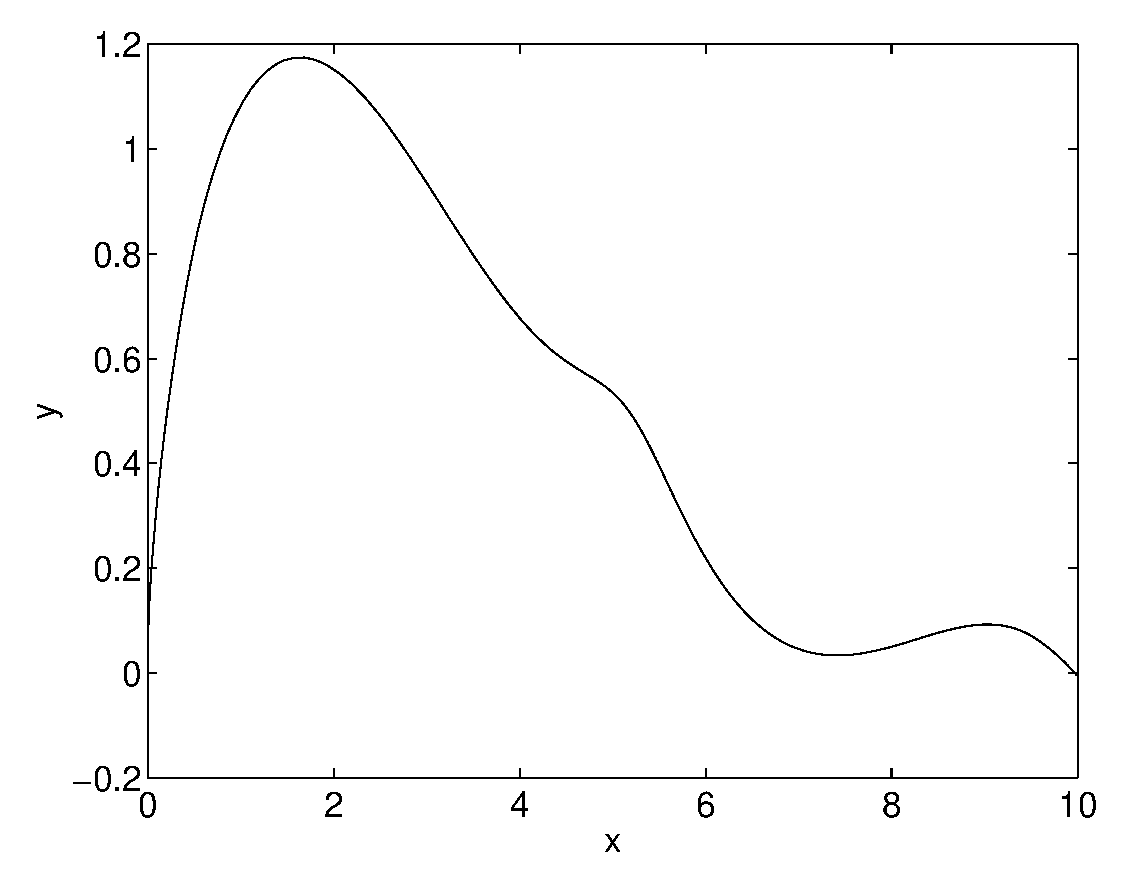
\includegraphics[width=\textwidth]{img/unicycle_path.eps}
\caption{path}
\end{subfigure}
~
\begin{subfigure}[b]{0.45\textwidth}
\centering
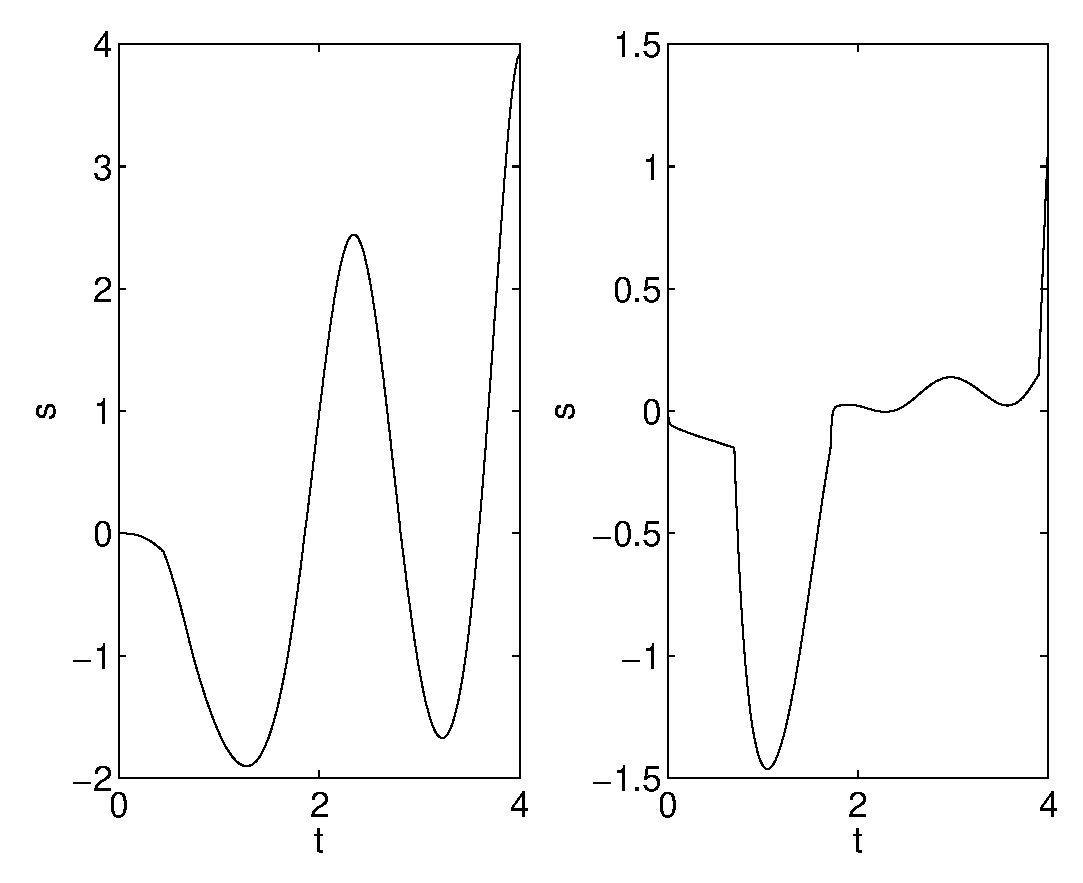
\includegraphics[width=\textwidth]{img/unicycle_slips.eps}
\caption{slips}
\end{subfigure}

\begin{subfigure}[b]{0.45\textwidth}
\centering
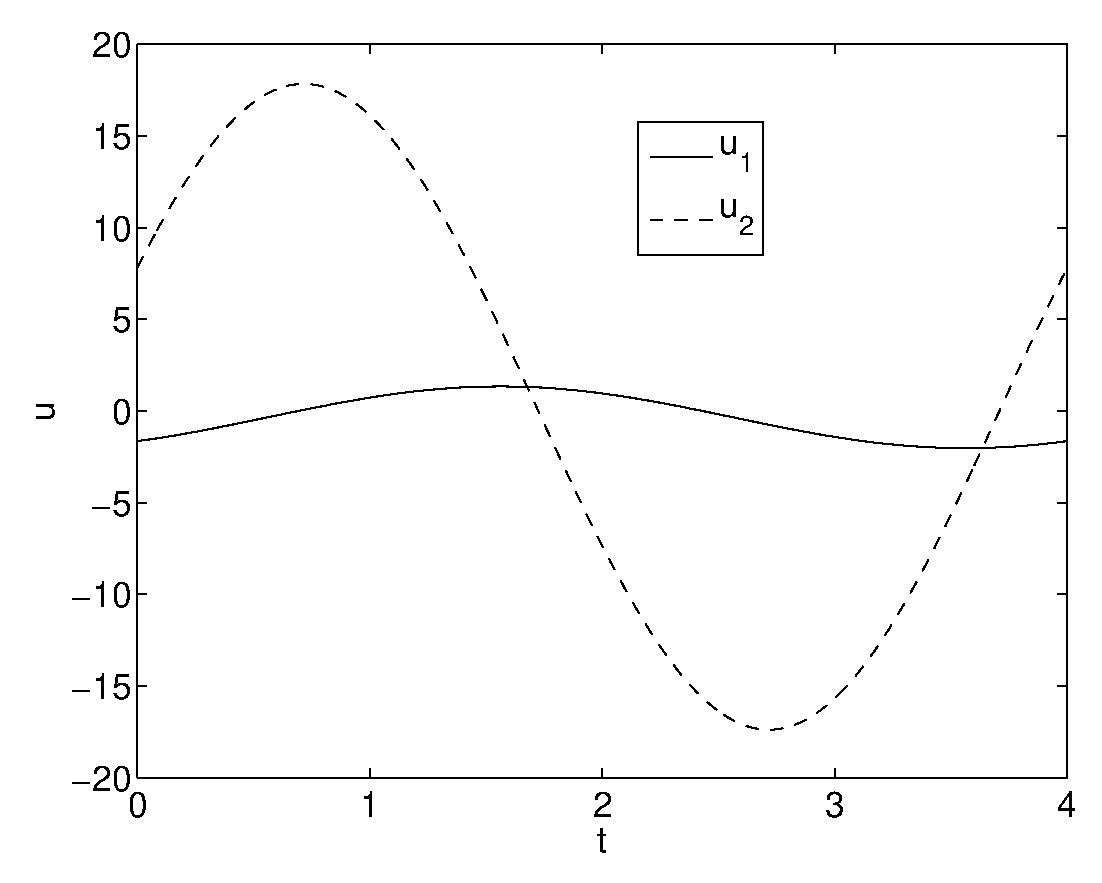
\includegraphics[width=\textwidth]{img/unicycle_u.eps}
\caption{control inputs}
\end{subfigure}
~
\begin{subfigure}[b]{0.45\textwidth}
\centering
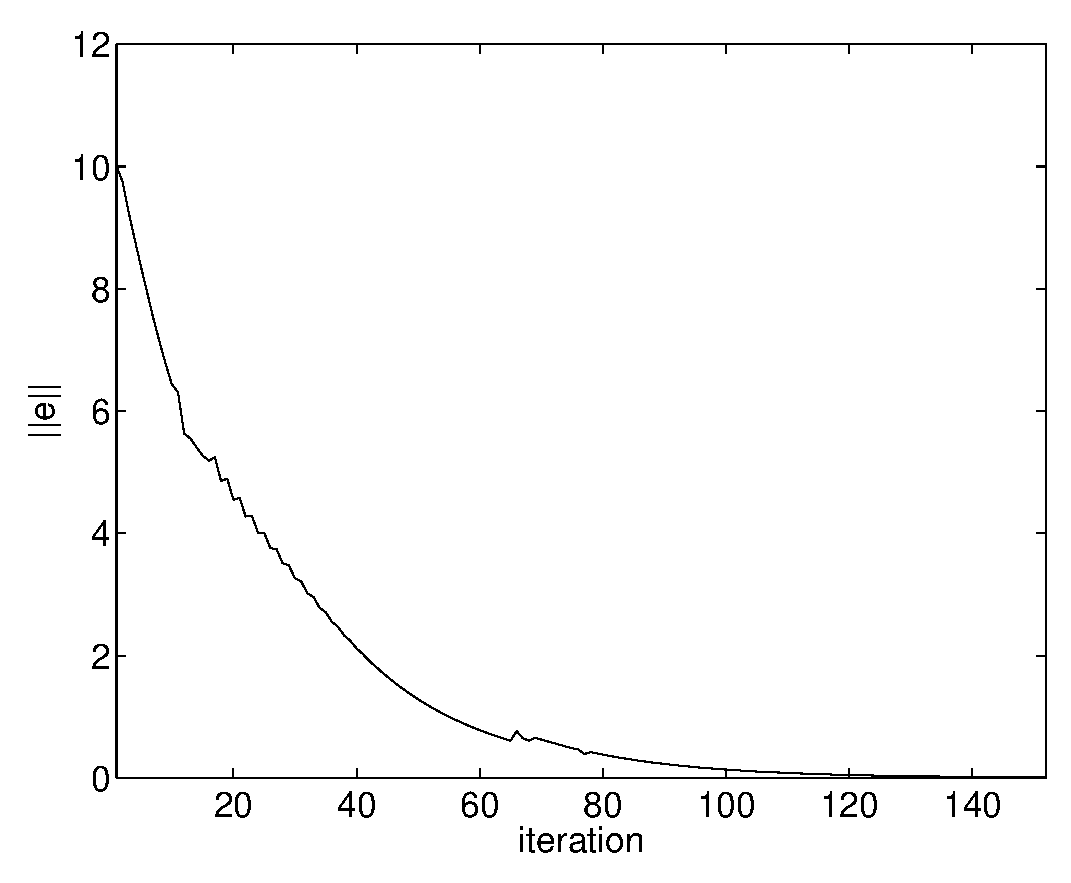
\includegraphics[width=\textwidth]{img/unicycle_err.eps}
\caption{error norm}
\end{subfigure}
\caption{Unicycle, discontinuous friction model}
\label{fig:pr_uni}
\end{figure}

\section{Mobile platform}
\subsection{Problem formulation}
\label{sec:rex_task}
The problem to be solved is to move the platform from the initial state
$q_0 = [w_0; \dot{w}_0] = (0, 0, a\frac{\pi}{2}, 0_7)^T$ to the desired state
$q_d = [w_d; \dot{w}_d] = (10, 0, a\frac{\pi}{2}, 0_7)^T$
within the given amount of time $T$. 
This corresponds to a parking manoeuvre.
%
%Now two types of friction models will be discussed --- linear
%and discontinuous. These models will be employed in simulations
%regarding solving the above problem.

\subsection{Simulation conditions}
\label{sec:pltf_params}
The object parameters were set according to \cite{coupled} and are as follows:
\begin{multicols}{2}
\begin{itemize}
\item $m_p = 21.107\,\mathrm{kg}$,
\item $m_w = 2.380\,\mathrm{kg}$,
\item $a_{p1} = 0.377\,\mathrm{m}$,
\item $a_{p2} = 0.008\,\mathrm{m}$,
\item $a = 0.730\,\mathrm{m}$,
\item $b = 0.350\,\mathrm{m}$,
\item $R = 0.127\,\mathrm{m}$,
\item $I_{p33} = 1.991\,\mathrm{kgm^2}$,
\item $I_{w11} = 0.015\,\mathrm{kgm^2}$,
\item $I_{w33} = 0.009\,\mathrm{kgm^2}$.
\end{itemize}
\end{multicols}
\setcounter{MaxMatrixCols}{14}
Initial conditions for the $\lambda$ parameters used to compute control functions
in \eqref{eq:endogen_num} are
\begin{equation}
\lambda_0=
(\underbrace{0, \ 0.5, \ 0, \ 0, \ 0, \ 0, \ 0,}_{u_1}\ \underbrace{0, \ 0.5, \ 0, \ 0, \ 0, \ 0, \ 0}_{u_2})^T,
\end{equation}
i.e. only first harmonic sines are used.
 	

\subsection{Linear friction model}
This model assumes that coefficients $\epsilon_i$ and $\tau_i$ in \eqref{eq:force_r} are constant. Four cases of friction coefficients values have been analysed:
\begin{enumerate}
\item $\epsilon_i=15$ and $\tau_i=15$,
\item $\epsilon_i=15$ and $\tau_i=1$,
\item $\epsilon_i=1$ and $\tau_i=15$,
\item $\epsilon_i=1$ and $\tau_i=1$,
\end{enumerate}
for $i=1,\,2,\,3,\,4$.
Every case was studied with two different time horizons 10\,s and 20\,s. The results of the simulations are shown in figures ...

It is also worth to check whether the input functions obtained through the algorithm are feasible on the real object. The total energy of the signal was computed as $\int_0^T u^2\ud t$ and the maximal amplitude which can be compared to the maximum torque achievable by the real actuator. These values computed for all the simulations run are presented in table \ref{tab:control}.
\begin{table}[h]
\centering
\caption{Control input functions parameters}
\label{tab:control}
\begin{tabular}{rrr|r|r|r|r|}
\cline{4-7}
\multicolumn{1}{c}{}                      & \multicolumn{1}{c}{}                     & \multicolumn{1}{c|}{}            & \multicolumn{2}{c|}{energy}                             & \multicolumn{2}{c|}{amplitude}                          \\ \hline
\multicolumn{1}{|c|}{$\tau$}              & \multicolumn{1}{c|}{$\epsilon$}          & \multicolumn{1}{c|}{$T$ {[}s{]}} & \multicolumn{1}{c|}{$u_1$} & \multicolumn{1}{c|}{$u_2$} & \multicolumn{1}{c|}{$u_1$} & \multicolumn{1}{c|}{$u_2$} \\ \hline
\multicolumn{1}{|r|}{\multirow{4}{*}{1}}  & \multicolumn{1}{r|}{\multirow{2}{*}{1}}  & 20                               & 5906                       & 805                        & 3.16                       & 1.26                       \\ \cline{3-7} 
\multicolumn{1}{|r|}{}                    & \multicolumn{1}{r|}{}                    & 10                               & 19337                      & 2036                       & 8.03                       & 3.09                       \\ \cline{2-7} 
\multicolumn{1}{|r|}{}                    & \multicolumn{1}{r|}{\multirow{2}{*}{15}} & 20                               & 118900                     & 21301                      & 14.07                      & 6.03                       \\ \cline{3-7} 
\multicolumn{1}{|r|}{}                    & \multicolumn{1}{r|}{}                    & 10                               & 662430                     & 309980                     & 48.38                      & 31.56                      \\ \hline
\multicolumn{1}{|r|}{\multirow{4}{*}{15}} & \multicolumn{1}{r|}{\multirow{2}{*}{1}}  & 20                               & 5906                       & 805                        & 3.16                       & 1.26                       \\ \cline{3-7} 
\multicolumn{1}{|r|}{}                    & \multicolumn{1}{r|}{}                    & 10                               & 19335                      & 2034                       & 8.03                       & 3.09                       \\ \cline{2-7} 
\multicolumn{1}{|r|}{}                    & \multicolumn{1}{r|}{\multirow{2}{*}{15}} & 20                               & 118900                     & 21298                      & 14.06                      & 6.00                       \\ \cline{3-7} 
\multicolumn{1}{|r|}{}                    & \multicolumn{1}{r|}{}                    & 10                               & 661100                     & 309080                     & 48.36                      & 31.56                      \\ \hline
\end{tabular}
\end{table}
\begin{figure}[h]
\begin{subfigure}[b]{\textwidth}
\centering
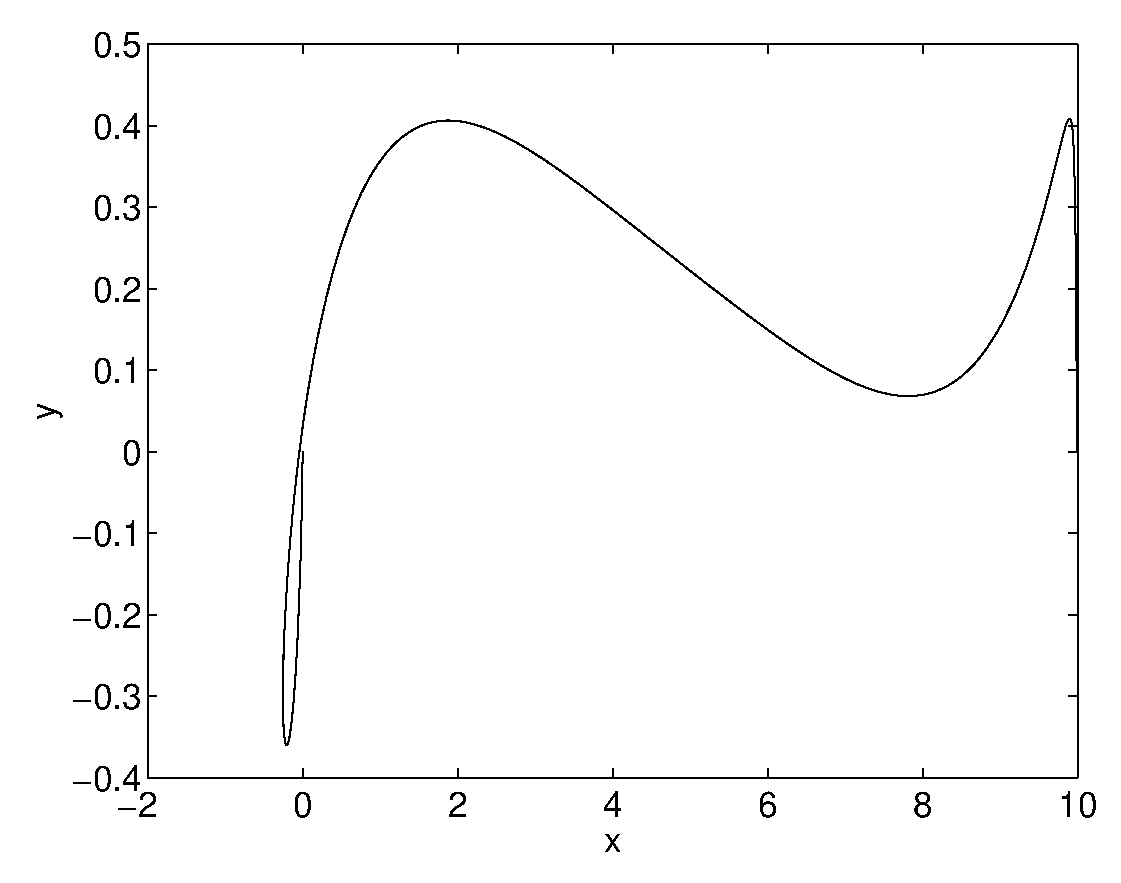
\includegraphics[height=0.3\textheight]{img/final_15_1_10_path.eps}
\caption{path}
\end{subfigure}

\begin{subfigure}[b]{\textwidth}
\centering
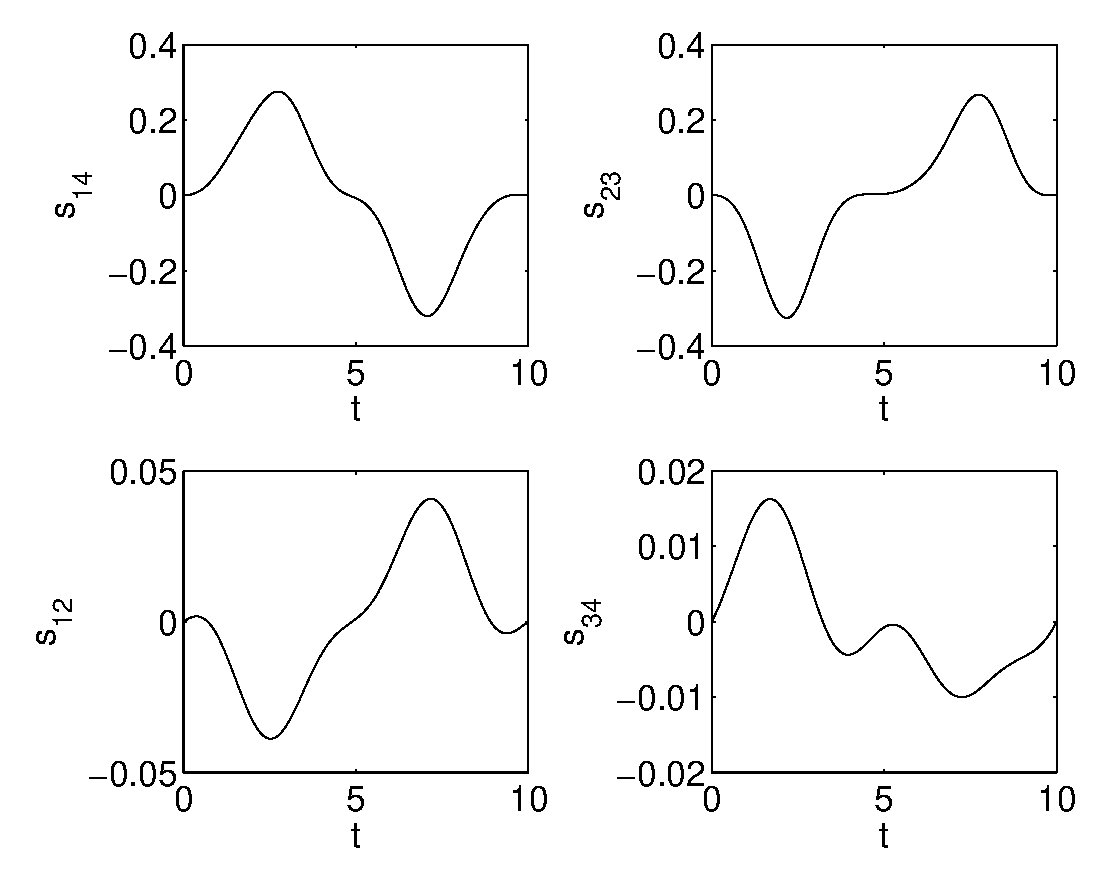
\includegraphics[height=0.3\textheight]{img/final_15_1_10_slips.eps}
\caption{slips}
\end{subfigure}

\begin{subfigure}[b]{\textwidth}
\centering
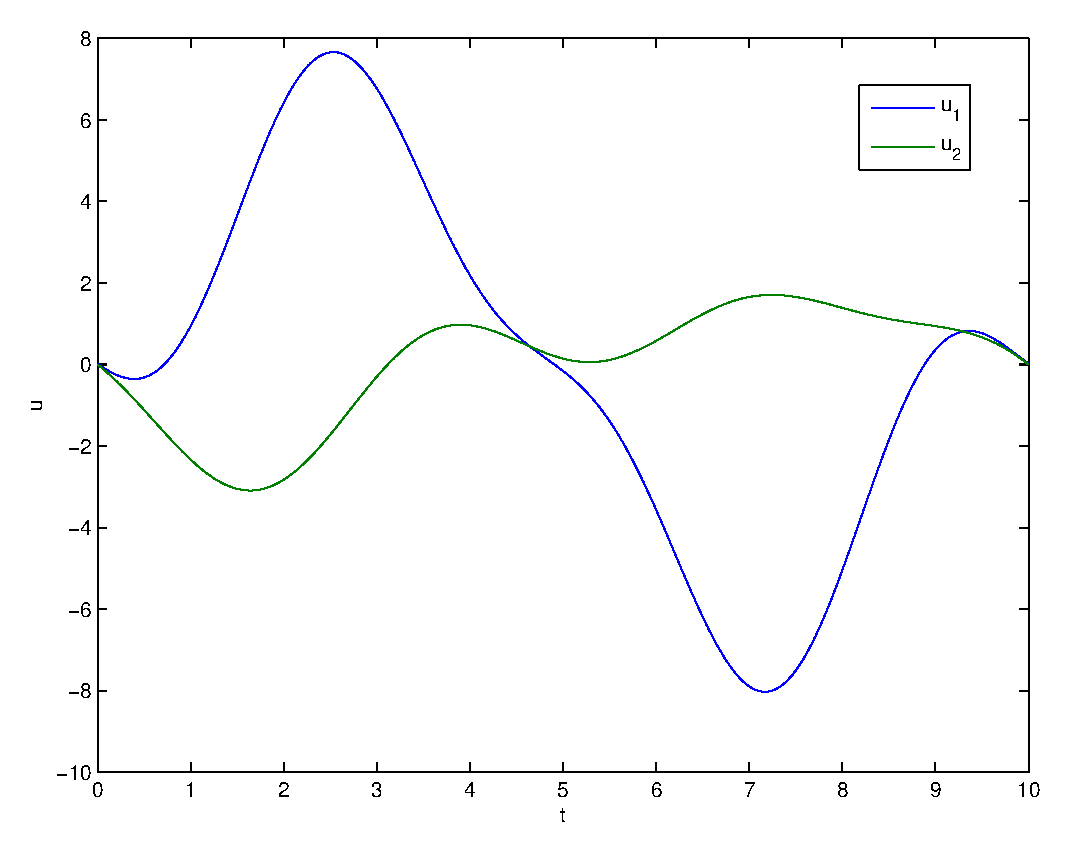
\includegraphics[height=0.3\textheight]{img/final_15_1_10_u.eps}
\caption{path}
\end{subfigure}
\caption{Mobile platform, $\epsilon=15$, $\tau=1$, $T=10$}
\label{fig:pl1}
\end{figure}

\begin{figure}[h]
\begin{subfigure}[b]{\textwidth}
\centering
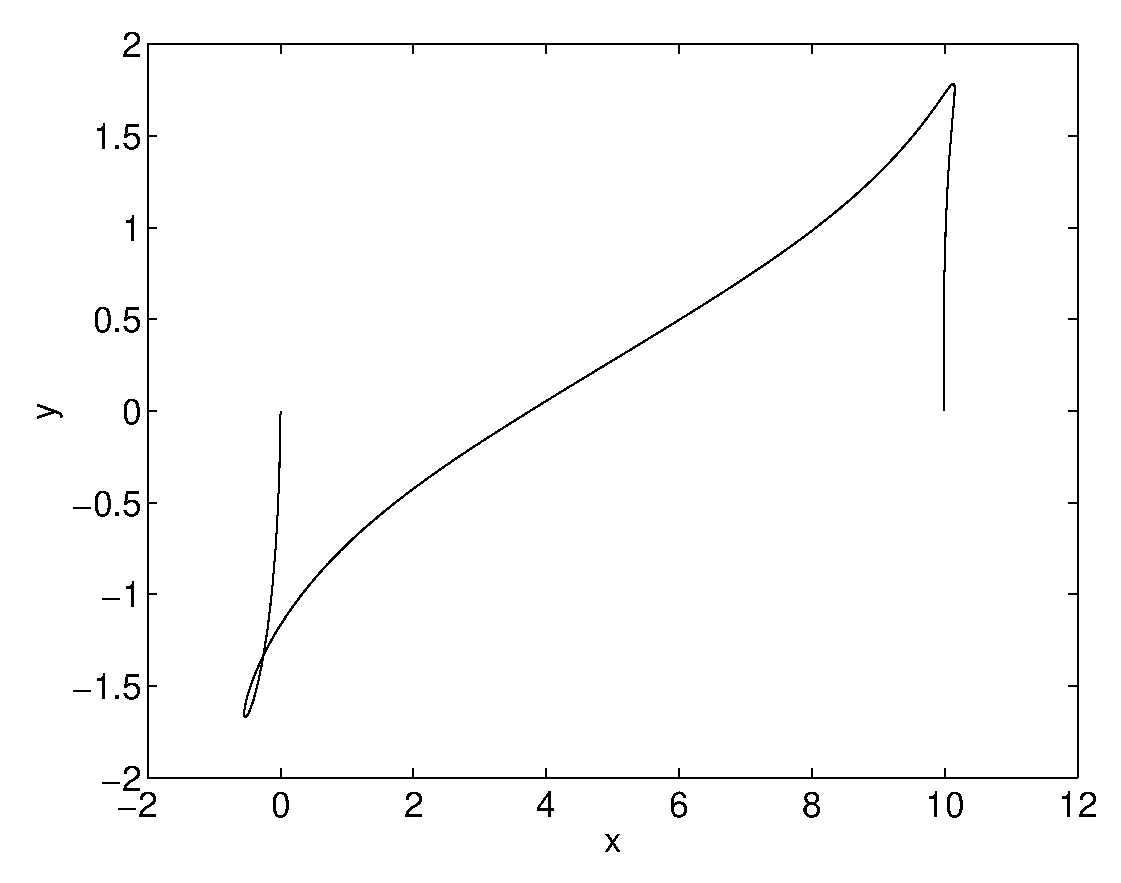
\includegraphics[height=0.3\textheight]{img/final_15_1_20_path.eps}
\caption{path}
\end{subfigure}

\begin{subfigure}[b]{\textwidth}
\centering
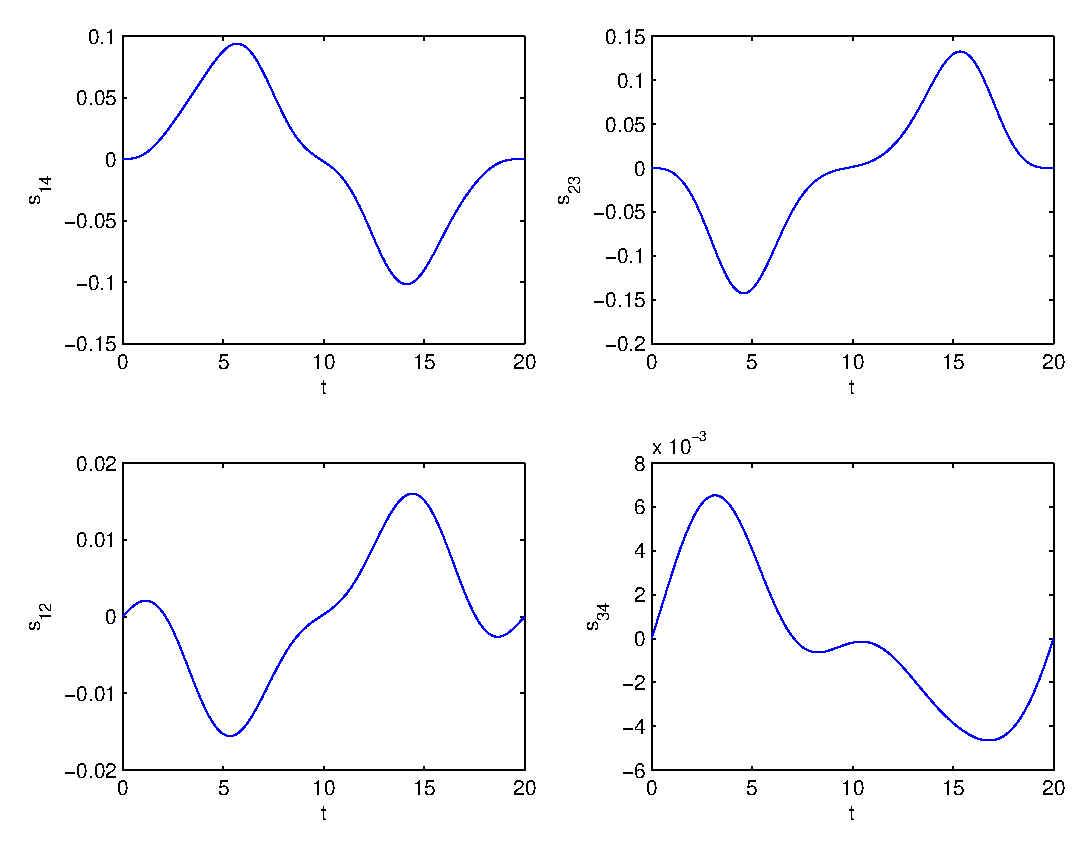
\includegraphics[height=0.3\textheight]{img/final_15_1_20_slips.eps}
\caption{slips}
\end{subfigure}

\begin{subfigure}[b]{\textwidth}
\centering
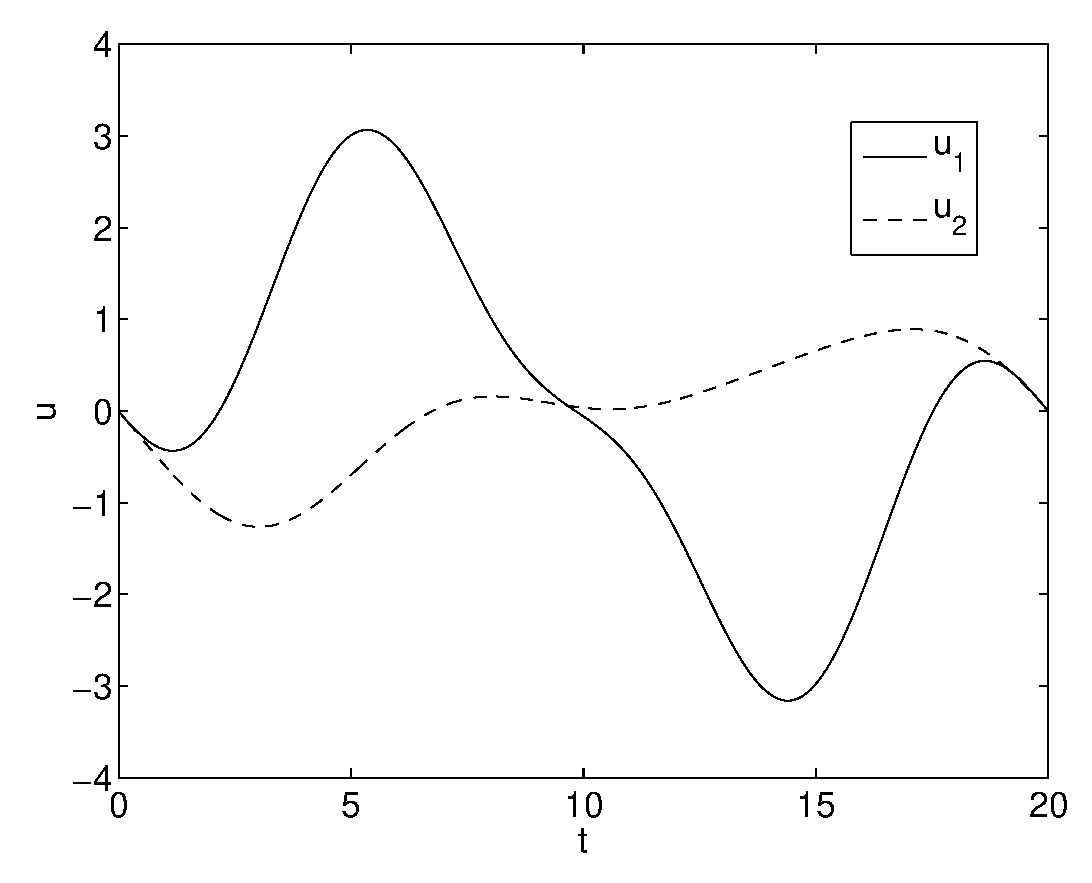
\includegraphics[height=0.3\textheight]{img/final_15_1_20_u.eps}
\caption{path}
\end{subfigure}
\caption{Mobile platform, $\epsilon=15$, $\tau=1$, $T=20$}
\label{fig:pl2}
\end{figure}

%%%%%%%%%%%%%%%%%%%%%%%%%%%%%%%%%%%%%%%%%%%%%%%%%%%%%%%%%%%%%%%%%%%%%%%%%%%%%%%%%%%%%%%%%%%
%%%%%%%%%%%%%%%%%%%%%%%%%%%%%%%%%%%%%%%%%%%%%%%%%%%%%%%%%%%%%%%%%%%%%%%%%%%%%%%%%%%%%%%%%%%
%%%%%%%%%%%%%%%%%%%%%%%%%%%%%%%%%%%%%%%%%%%%%%%%%%%%%%%%%%%%%%%%%%%%%%%%%%%%%%%%%%%%%%%%%%%
%%%%%%%%%%%%%%%%%%%%%%%%%%%%%%%%%%%%%%%%%%%%%%%%%%%%%%%%%%%%%%%%%%%%%%%%%%%%%%%%%%%%%%%%%%%
%%%%%%%%%%%%%%%%%%%%%%%%%%%%%%%%%%%%%%%%%%%%%%%%%%%%%%%%%%%%%%%%%%%%%%%%%%%%%%%%%%%%%%%%%%%

\begin{figure}[h]
\begin{subfigure}[b]{\textwidth}
\centering
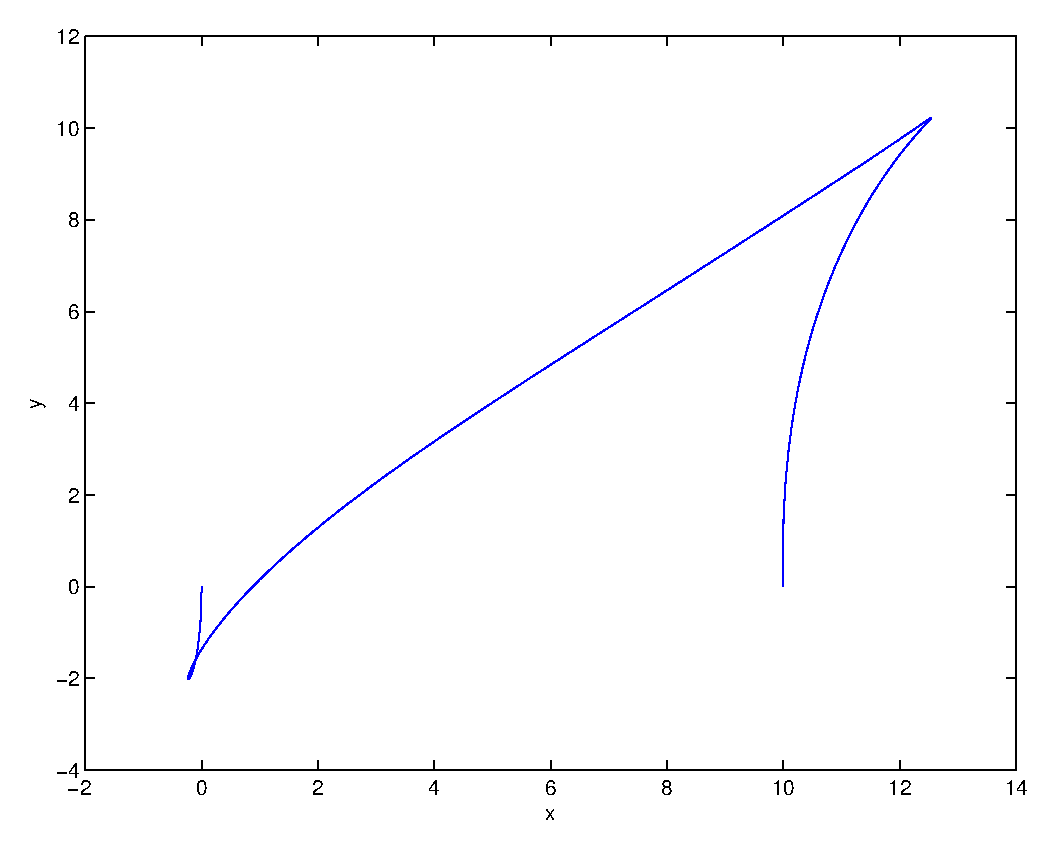
\includegraphics[height=0.3\textheight]{img/final_15_15_10_path.eps}
\caption{path}
\end{subfigure}

\begin{subfigure}[b]{\textwidth}
\centering
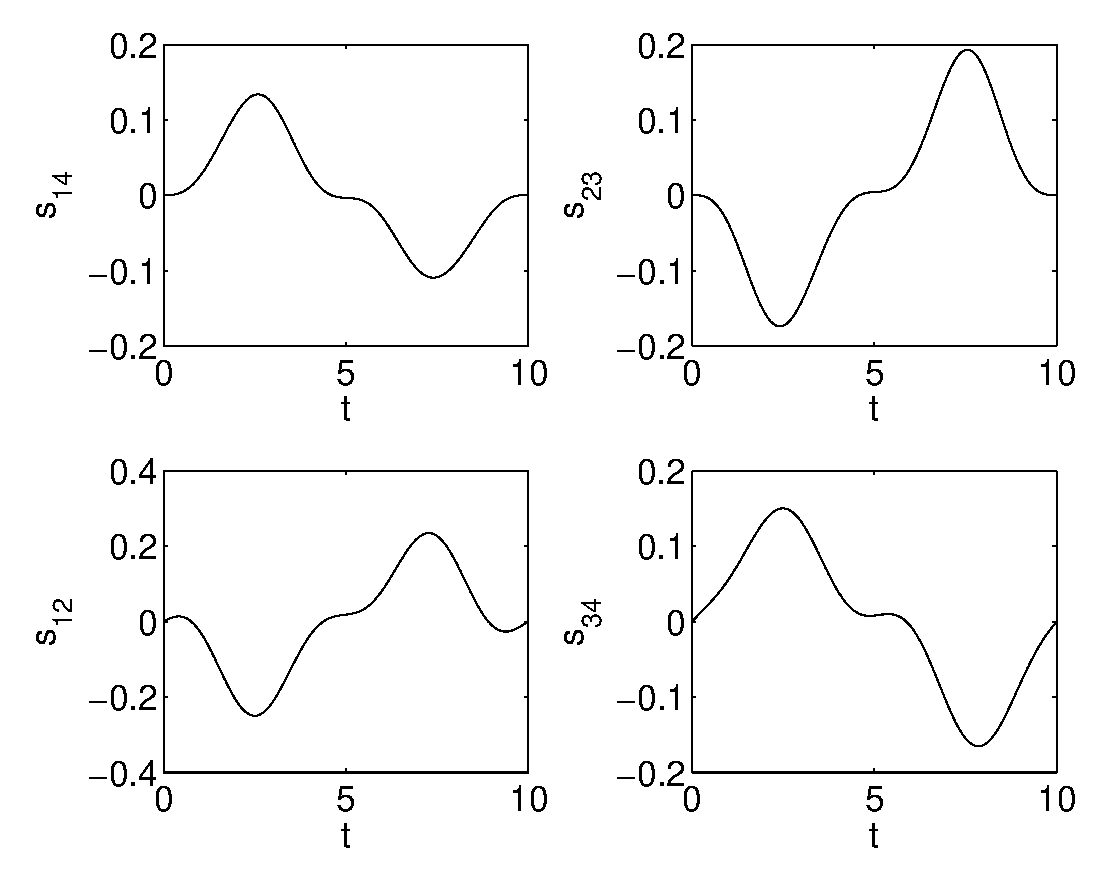
\includegraphics[height=0.3\textheight]{img/final_15_15_10_slips.eps}
\caption{slips}
\end{subfigure}

\begin{subfigure}[b]{\textwidth}
\centering
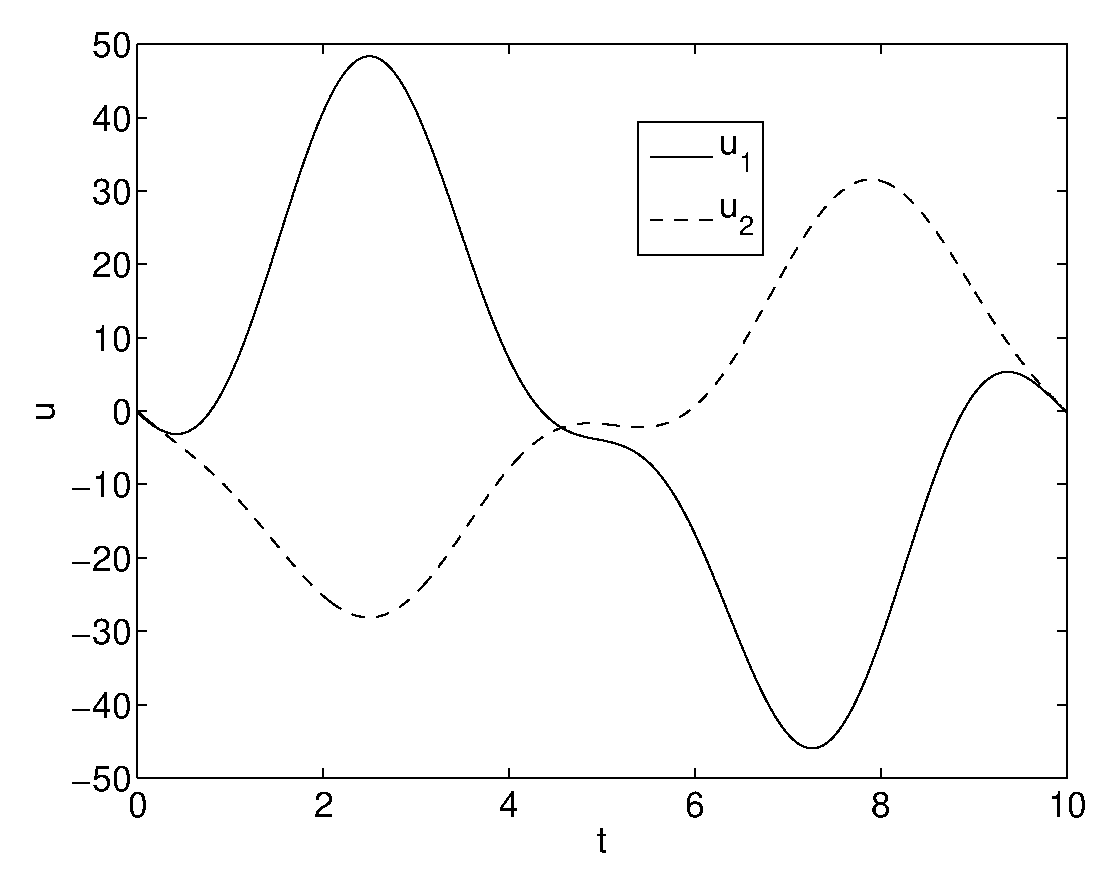
\includegraphics[height=0.3\textheight]{img/final_15_15_10_u.eps}
\caption{path}
\end{subfigure}
\caption{Mobile platform, $\epsilon=15$, $\tau=15$, $T=10$}
\label{fig:pl3}
\end{figure}

\begin{figure}[h]
\begin{subfigure}[b]{\textwidth}
\centering
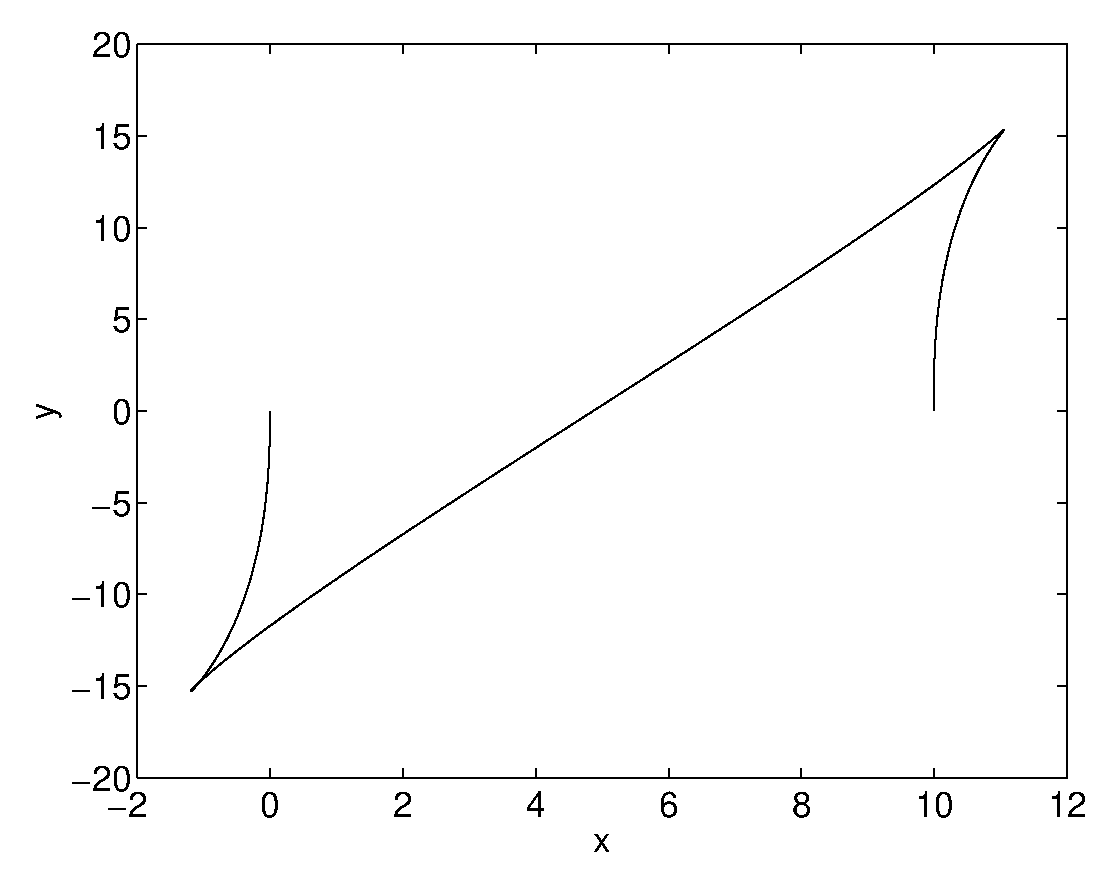
\includegraphics[height=0.3\textheight]{img/final_15_15_20_path.eps}
\caption{path}
\end{subfigure}

\begin{subfigure}[b]{\textwidth}
\centering
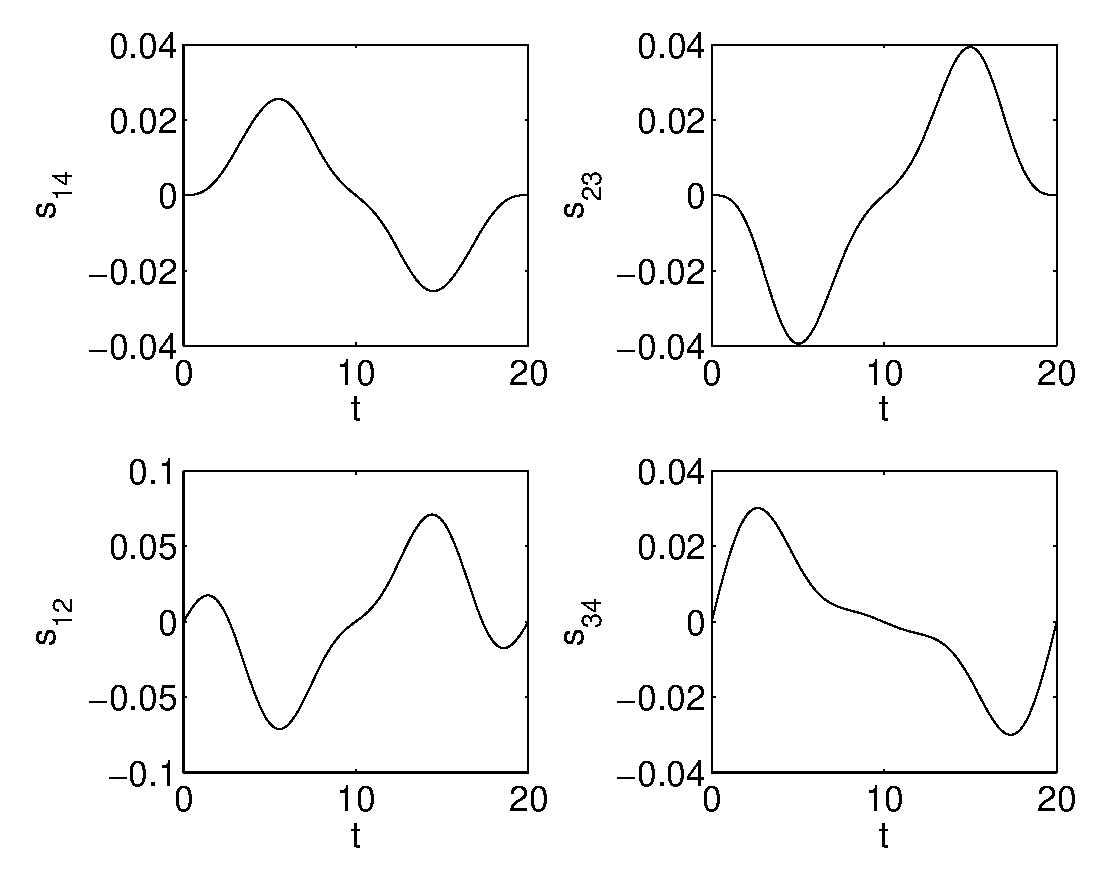
\includegraphics[height=0.3\textheight]{img/final_15_15_20_slips.eps}
\caption{slips}
\end{subfigure}

\begin{subfigure}[b]{\textwidth}
\centering
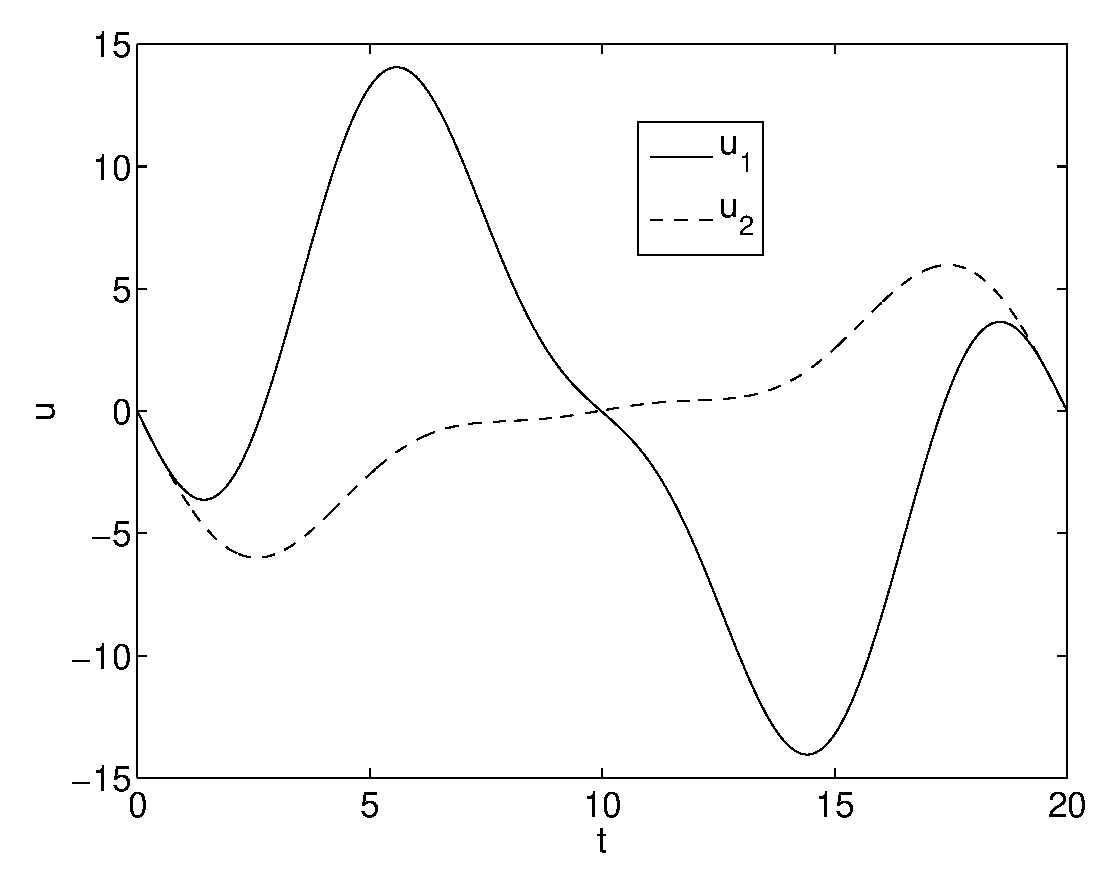
\includegraphics[height=0.3\textheight]{img/final_15_15_20_u.eps}
\caption{path}
\end{subfigure}
\caption{Mobile platform, $\epsilon=15$, $\tau=15$, $T=20$}
\label{fig:pl4}
\end{figure}

%%%%%%%%%%%%%%%%%%%%%%%%%%%%%%%%%%%%%%%%%%%%%%%%%%%%%%%%%%%%%%%%%%%%%%%%%%%%%%%%%%%%%%%%%%%
%%%%%%%%%%%%%%%%%%%%%%%%%%%%%%%%%%%%%%%%%%%%%%%%%%%%%%%%%%%%%%%%%%%%%%%%%%%%%%%%%%%%%%%%%%%
%%%%%%%%%%%%%%%%%%%%%%%%%%%%%%%%%%%%%%%%%%%%%%%%%%%%%%%%%%%%%%%%%%%%%%%%%%%%%%%%%%%%%%%%%%%
%%%%%%%%%%%%%%%%%%%%%%%%%%%%%%%%%%%%%%%%%%%%%%%%%%%%%%%%%%%%%%%%%%%%%%%%%%%%%%%%%%%%%%%%%%%
%%%%%%%%%%%%%%%%%%%%%%%%%%%%%%%%%%%%%%%%%%%%%%%%%%%%%%%%%%%%%%%%%%%%%%%%%%%%%%%%%%%%%%%%%%%
\begin{figure}[h]
\begin{subfigure}[b]{\textwidth}
\centering
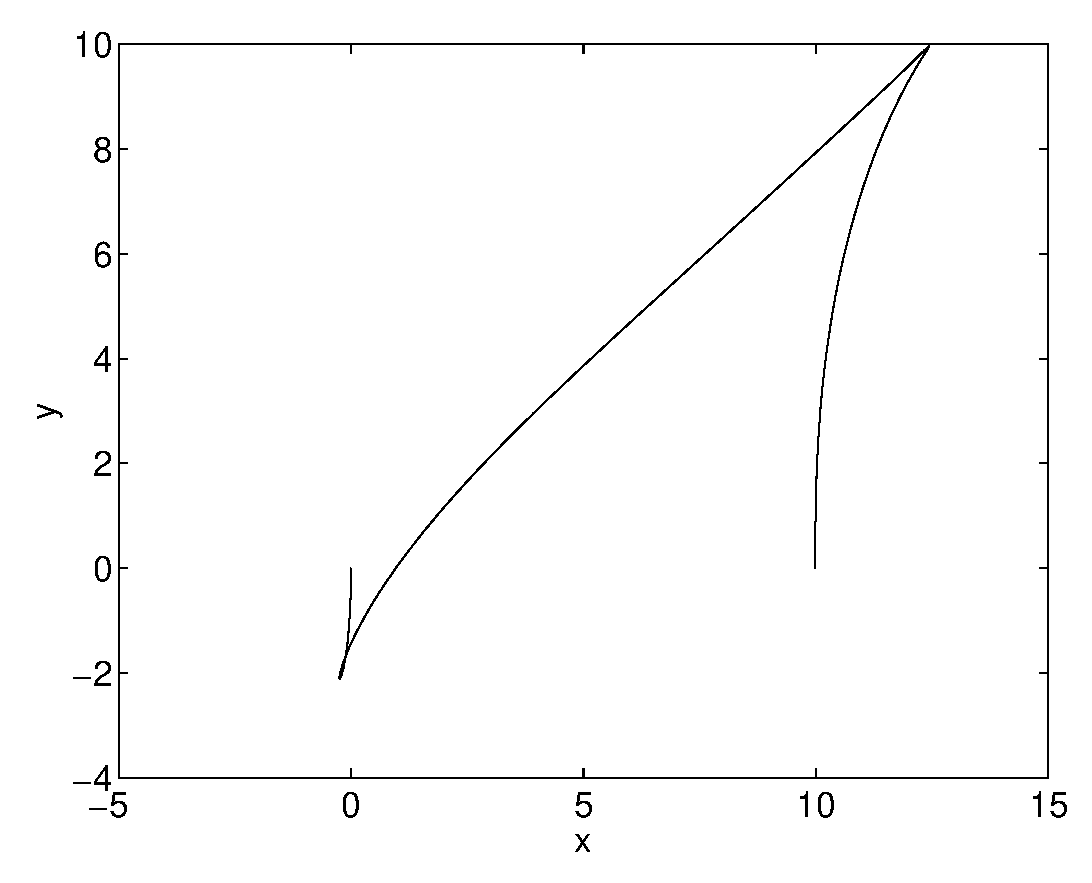
\includegraphics[height=0.3\textheight]{img/final_1_15_10_path.eps}
\caption{path}
\end{subfigure}

\begin{subfigure}[b]{\textwidth}
\centering
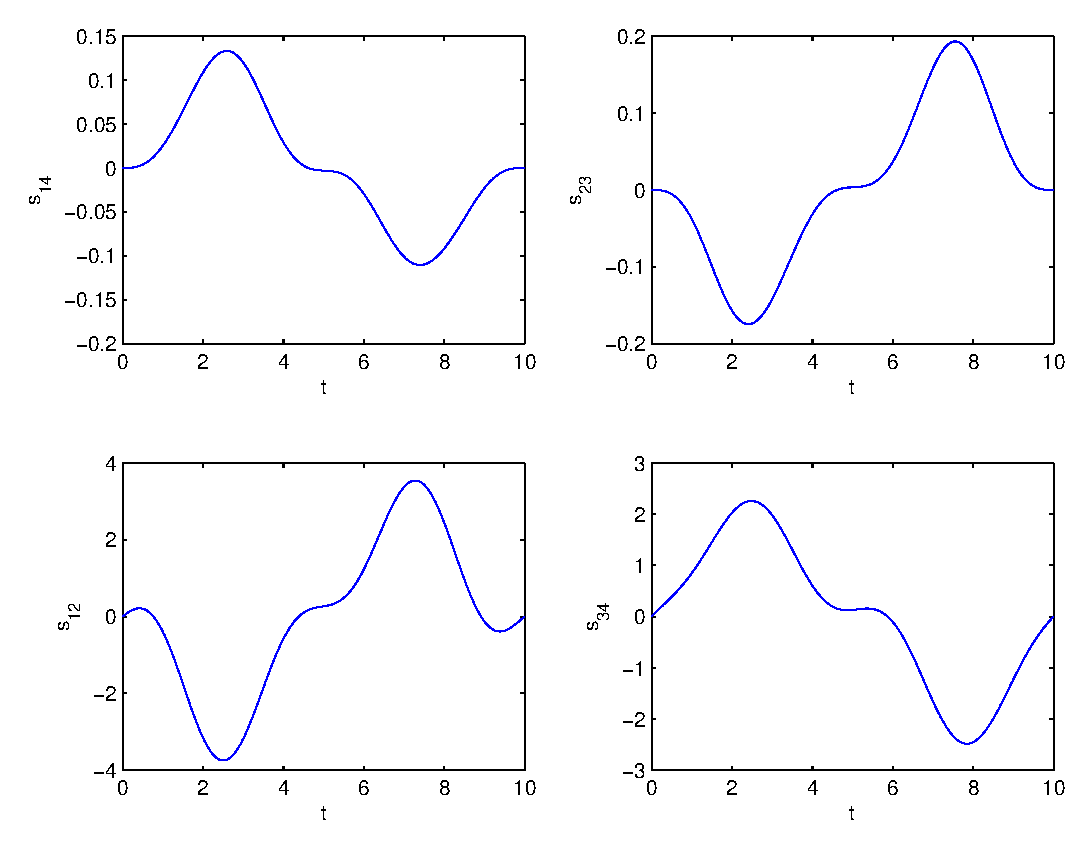
\includegraphics[height=0.3\textheight]{img/final_1_15_10_slips.eps}
\caption{slips}
\end{subfigure}

\begin{subfigure}[b]{\textwidth}
\centering
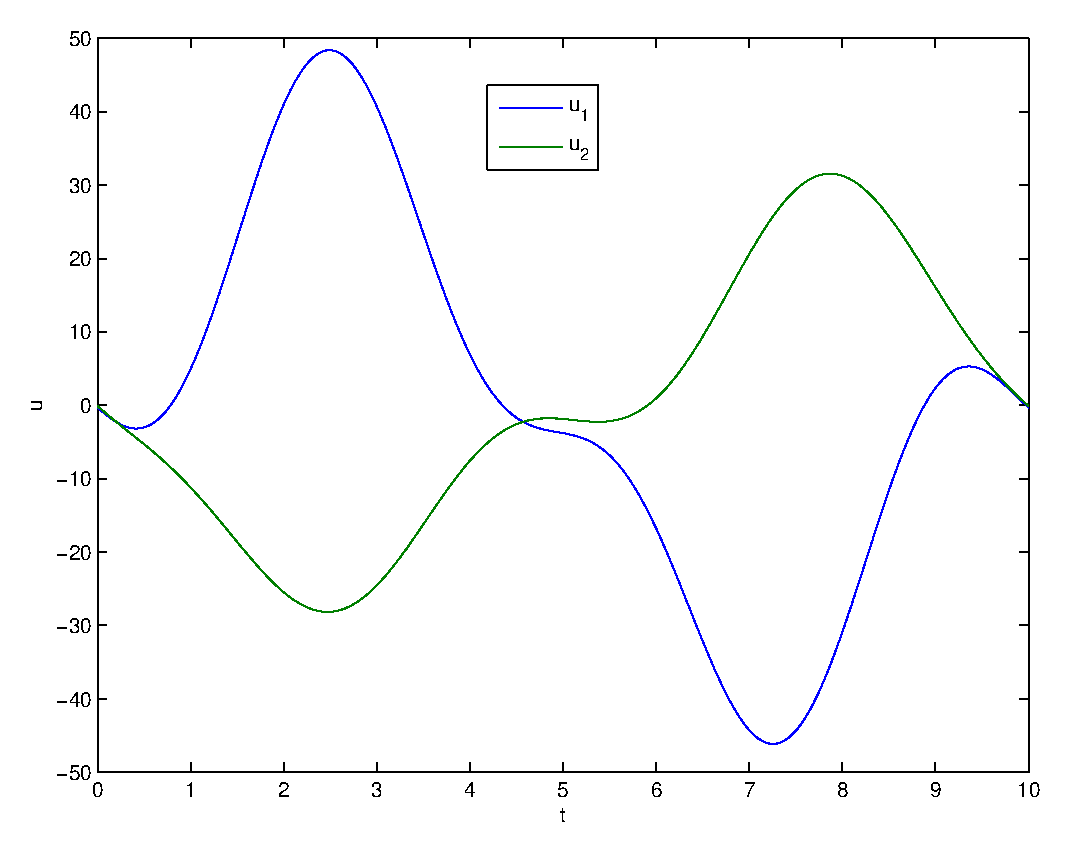
\includegraphics[height=0.3\textheight]{img/final_1_15_10_u.eps}
\caption{path}
\end{subfigure}
\caption{Mobile platform, $\epsilon=1$, $\tau=15$, $T=10$}
\label{fig:pl5}
\end{figure}

\begin{figure}[h]
\begin{subfigure}[b]{\textwidth}
\centering
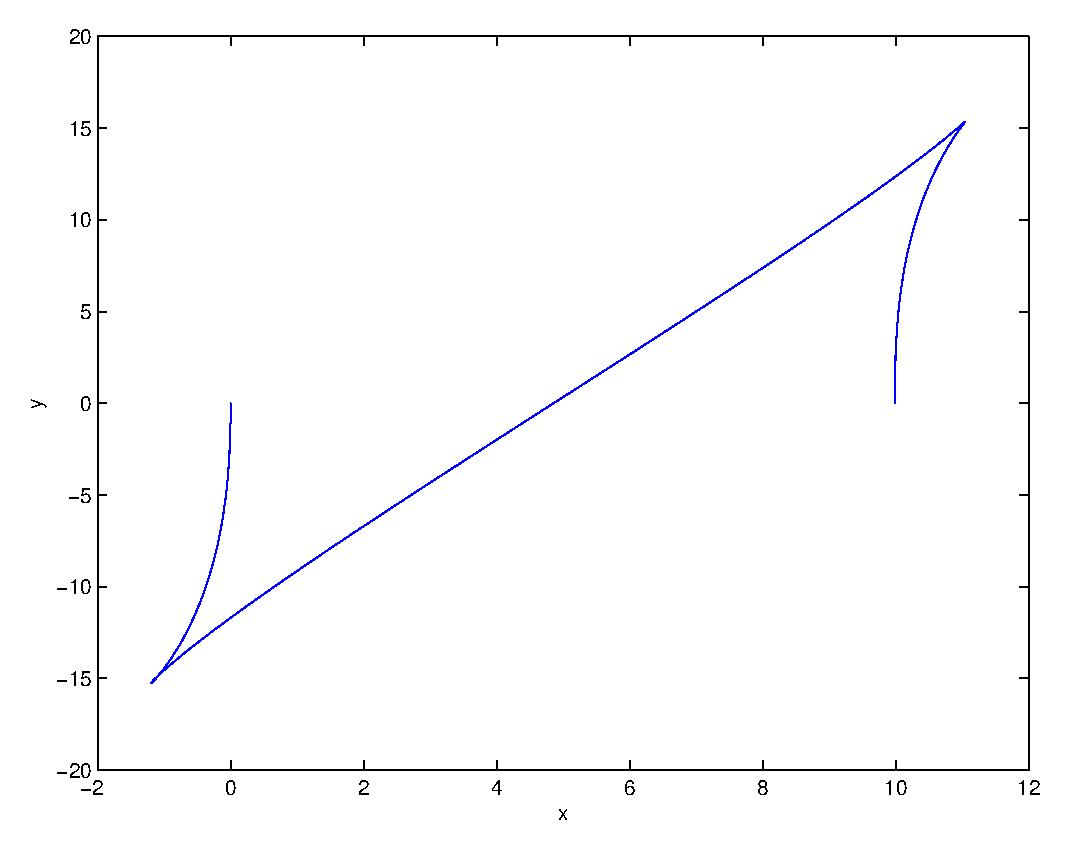
\includegraphics[height=0.3\textheight]{img/final_1_15_20_path.eps}
\caption{path}
\end{subfigure}

\begin{subfigure}[b]{\textwidth}
\centering
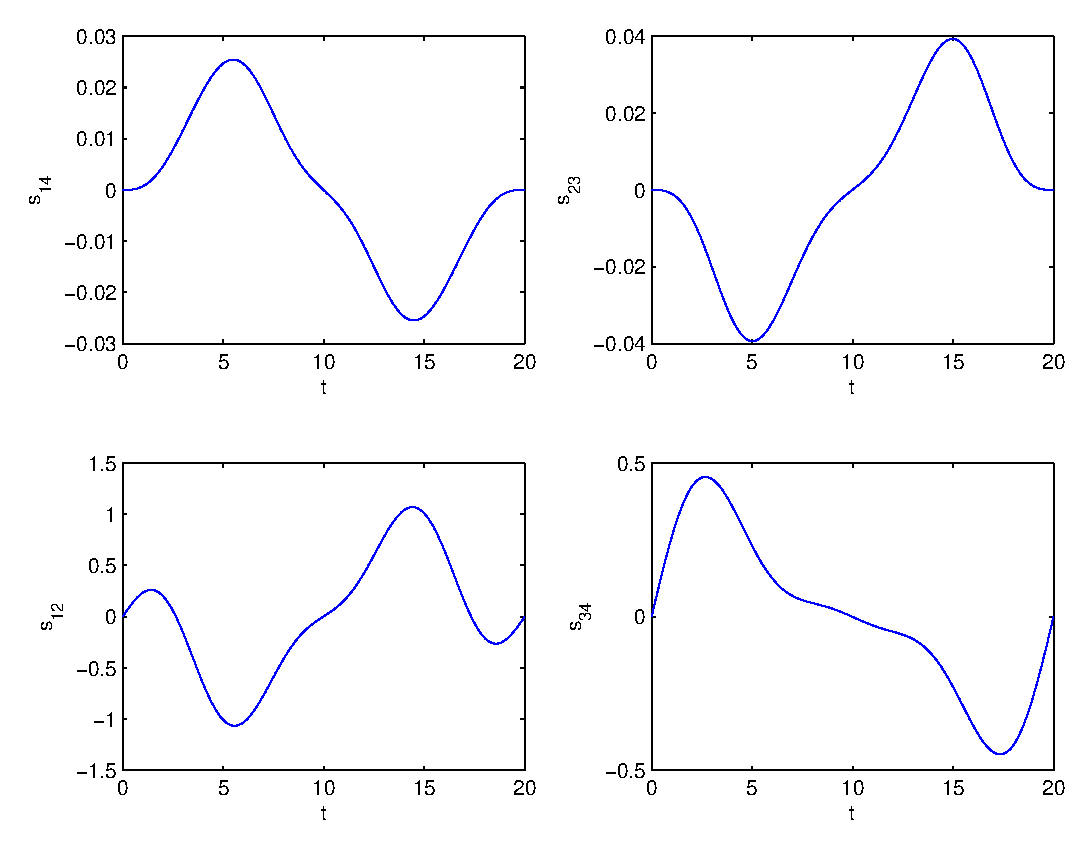
\includegraphics[height=0.3\textheight]{img/final_1_15_20_slips.eps}
\caption{slips}
\end{subfigure}

\begin{subfigure}[b]{\textwidth}
\centering
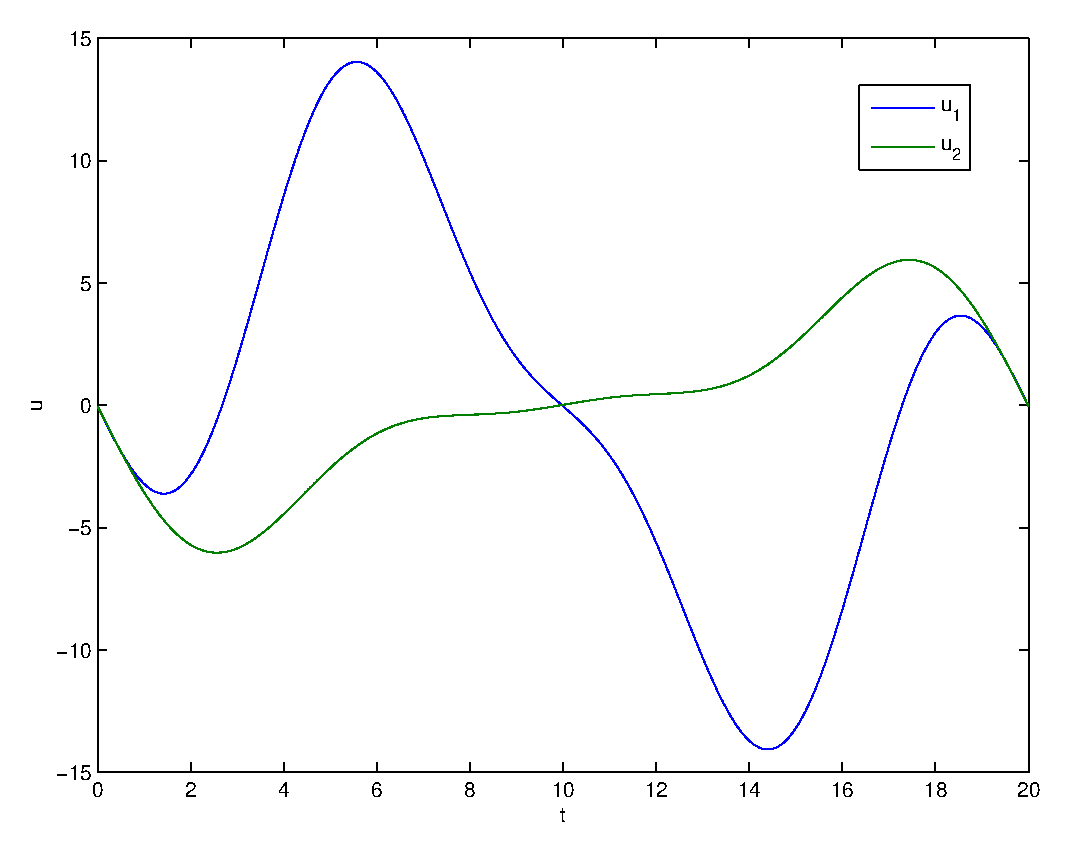
\includegraphics[height=0.3\textheight]{img/final_1_15_20_u.eps}
\caption{path}
\end{subfigure}
\caption{Mobile platform, $\epsilon=1$, $\tau=15$, $T=20$}
\label{fig:pl6}
\end{figure}

%%%%%%%%%%%%%%%%%%%%%%%%%%%%%%%%%%%%%%%%%%%%%%%%%%%%%%%%%%%%%%%%%%%%%%%%%%%%%%%%%%%%%%%%%%%
%%%%%%%%%%%%%%%%%%%%%%%%%%%%%%%%%%%%%%%%%%%%%%%%%%%%%%%%%%%%%%%%%%%%%%%%%%%%%%%%%%%%%%%%%%%
%%%%%%%%%%%%%%%%%%%%%%%%%%%%%%%%%%%%%%%%%%%%%%%%%%%%%%%%%%%%%%%%%%%%%%%%%%%%%%%%%%%%%%%%%%%
%%%%%%%%%%%%%%%%%%%%%%%%%%%%%%%%%%%%%%%%%%%%%%%%%%%%%%%%%%%%%%%%%%%%%%%%%%%%%%%%%%%%%%%%%%%
%%%%%%%%%%%%%%%%%%%%%%%%%%%%%%%%%%%%%%%%%%%%%%%%%%%%%%%%%%%%%%%%%%%%%%%%%%%%%%%%%%%%%%%%%%%
\begin{figure}[h]
\begin{subfigure}[b]{\textwidth}
\centering
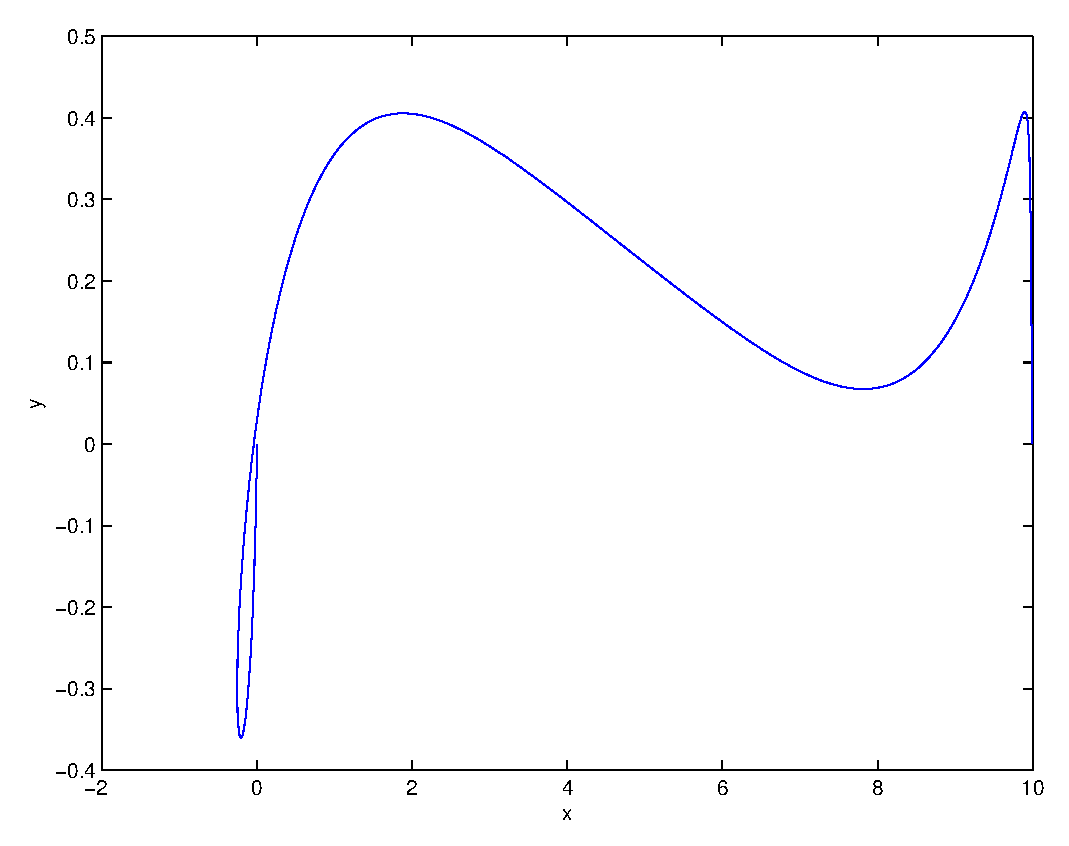
\includegraphics[height=0.3\textheight]{img/final_1_1_10_path.eps}
\caption{path}
\end{subfigure}

\begin{subfigure}[b]{\textwidth}
\centering
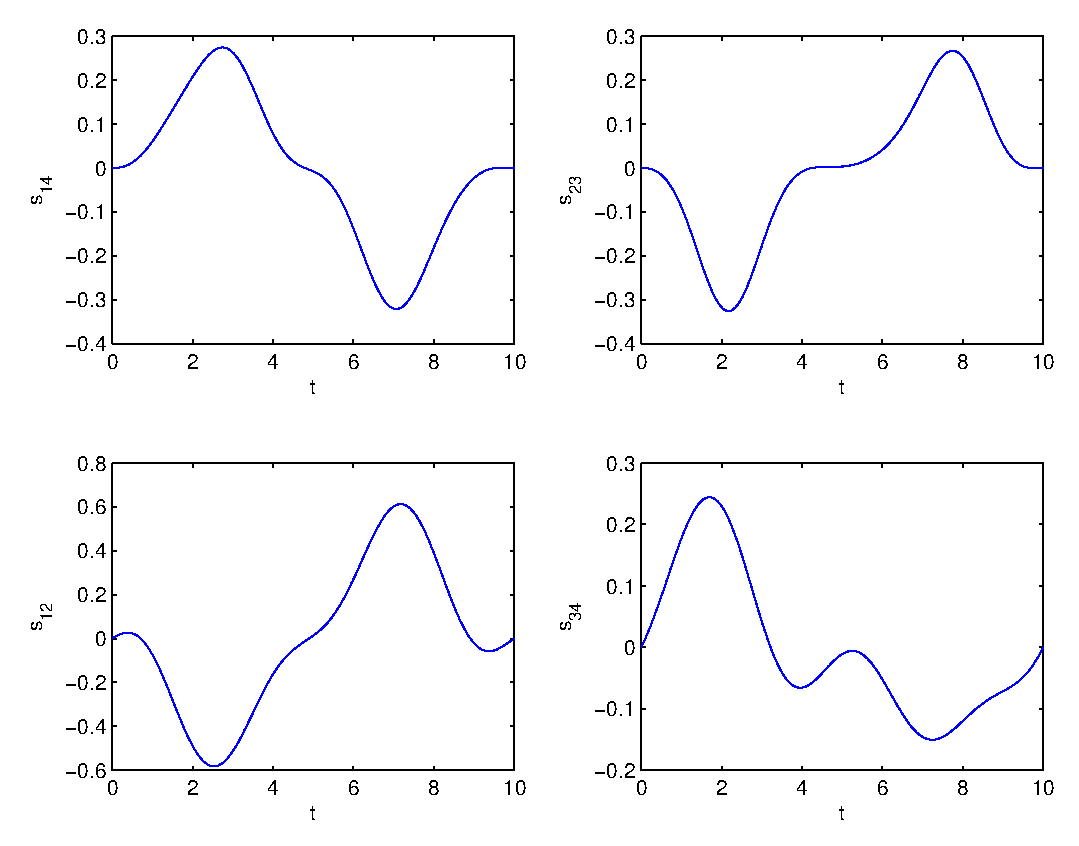
\includegraphics[height=0.3\textheight]{img/final_1_1_10_slips.eps}
\caption{slips}
\end{subfigure}

\begin{subfigure}[b]{\textwidth}
\centering
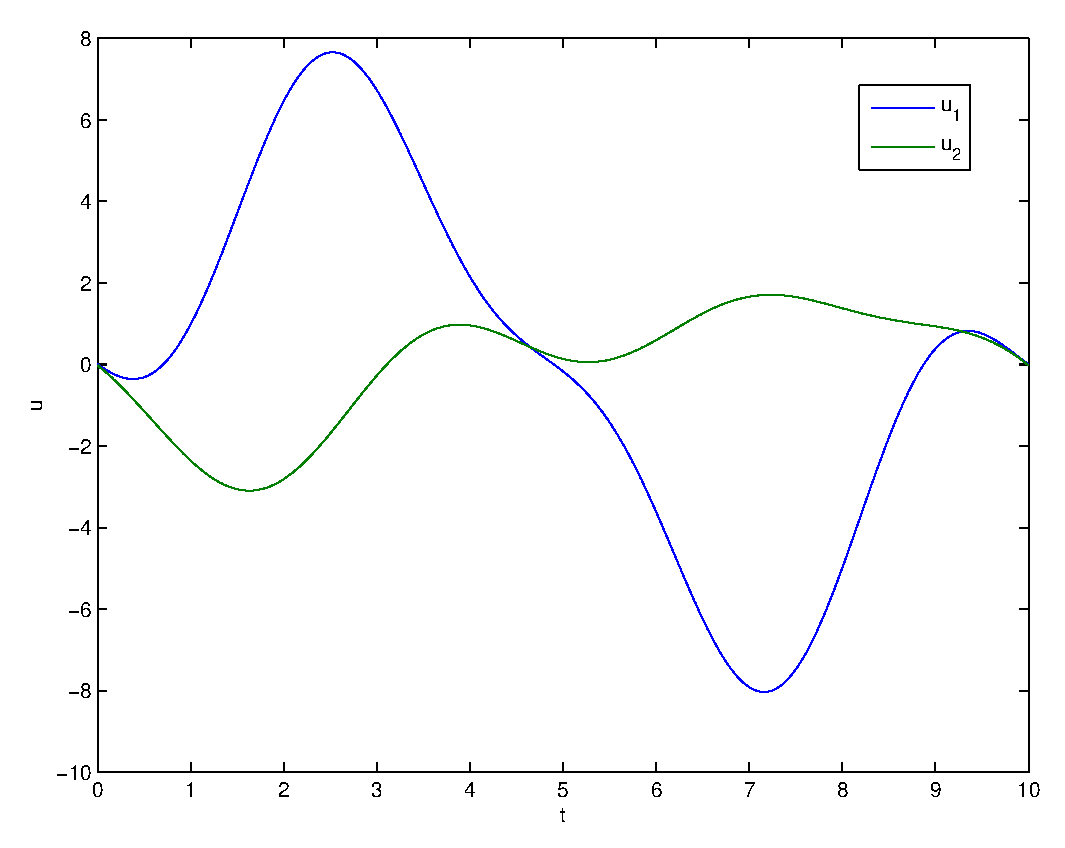
\includegraphics[height=0.3\textheight]{img/final_1_1_10_u.eps}
\caption{path}
\end{subfigure}
\caption{Mobile platform, $\epsilon=1$, $\tau=1$, $T=10$}
\label{fig:pl7}
\end{figure}

\begin{figure}[h]
\begin{subfigure}[b]{\textwidth}
\centering
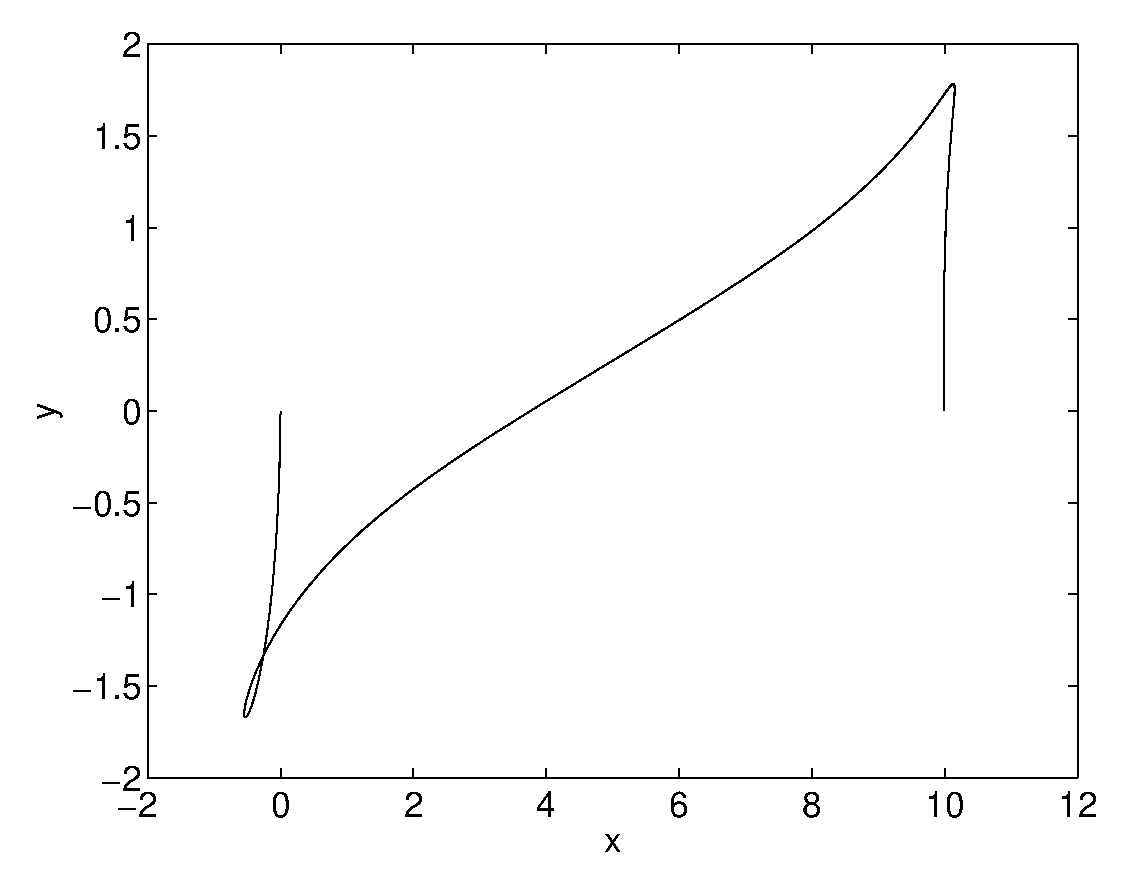
\includegraphics[height=0.3\textheight]{img/final_1_1_20_path.eps}
\caption{path}
\end{subfigure}

\begin{subfigure}[b]{\textwidth}
\centering
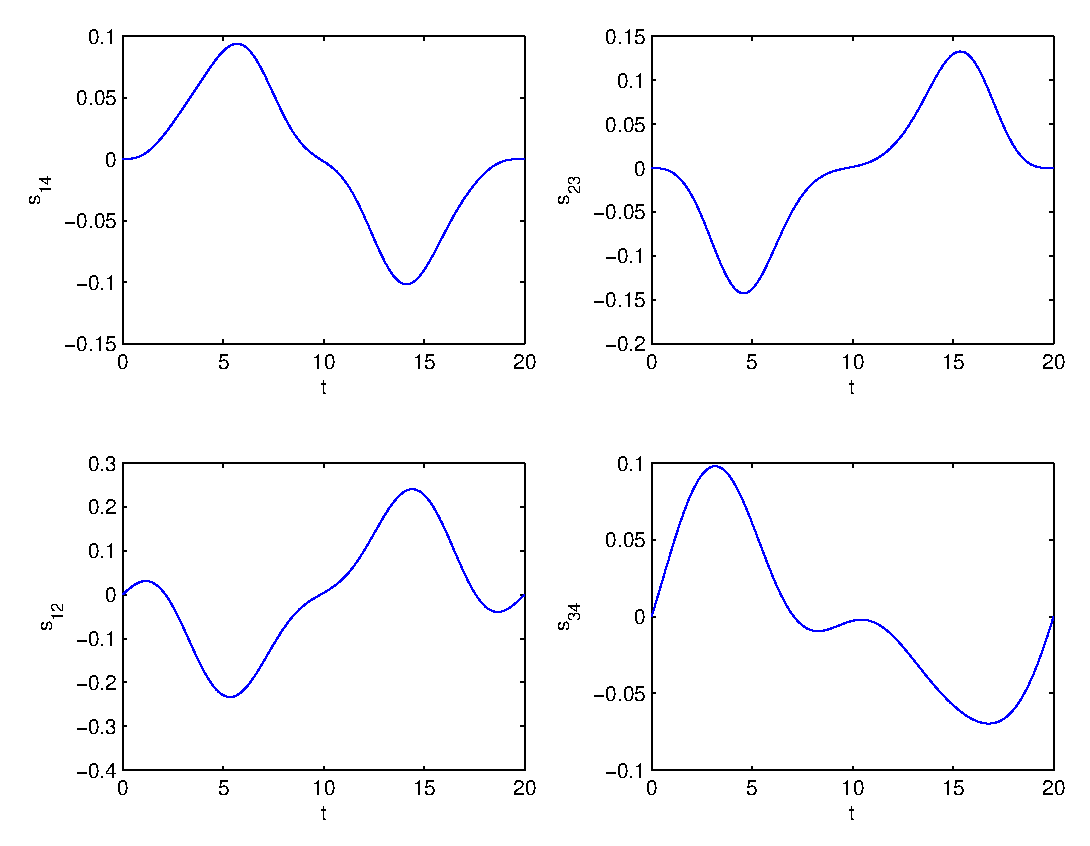
\includegraphics[height=0.3\textheight]{img/final_1_1_20_slips.eps}
\caption{slips}
\end{subfigure}

\begin{subfigure}[b]{\textwidth}
\centering
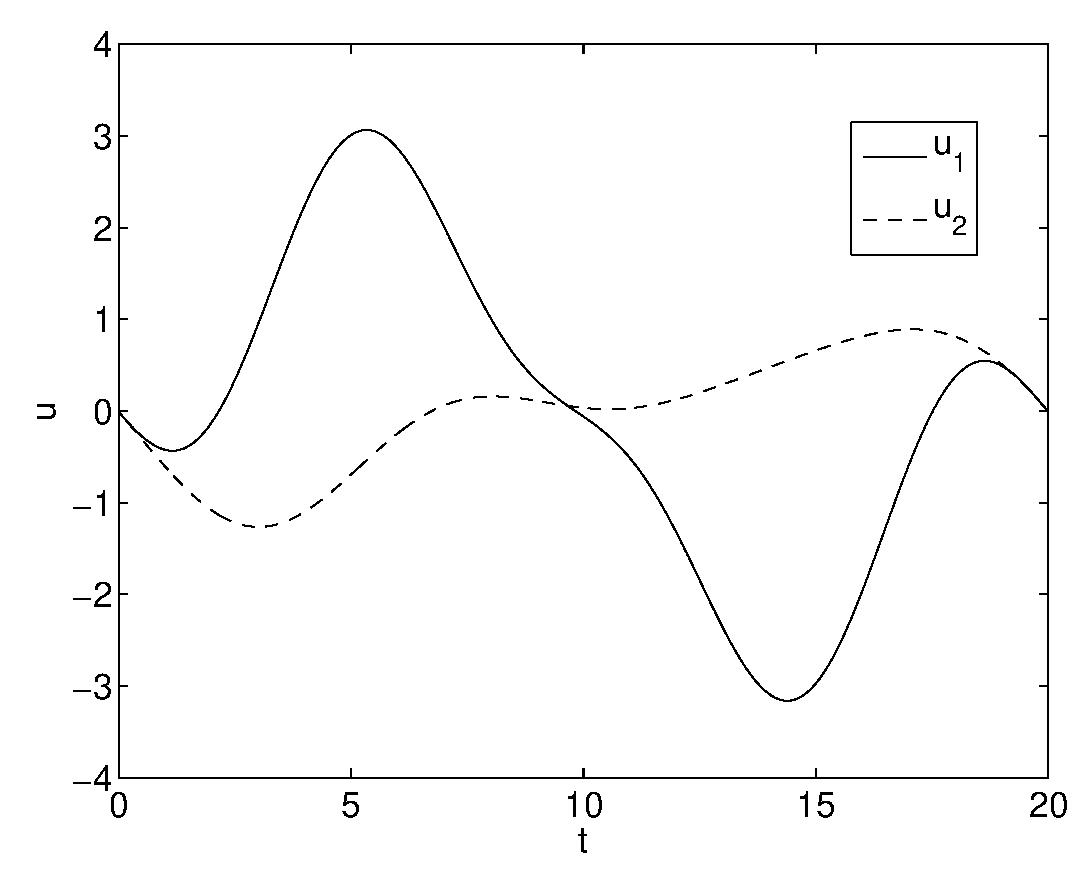
\includegraphics[height=0.3\textheight]{img/final_1_1_20_u.eps}
\caption{path}
\end{subfigure}
\caption{Mobile platform, $\epsilon=1$, $\tau=1$, $T=20$}
\label{fig:pl8}
\end{figure}

%%%%%%%%%%%%%%%%%%%%%%%%%%%%%%%%%%%%%%%%%%%%%%%%%%%%%%%%%%%%%%%%%%%%%%%%%%%%%%%%%%%%%%%%%%%
%%%%%%%%%%%%%%%%%%%%%%%%%%%%%%%%%%%%%%%%%%%%%%%%%%%%%%%%%%%%%%%%%%%%%%%%%%%%%%%%%%%%%%%%%%%
%%%%%%%%%%%%%%%%%%%%%%%%%%%%%%%%%%%%%%%%%%%%%%%%%%%%%%%%%%%%%%%%%%%%%%%%%%%%%%%%%%%%%%%%%%%
%%%%%%%%%%%%%%%%%%%%%%%%%%%%%%%%%%%%%%%%%%%%%%%%%%%%%%%%%%%%%%%%%%%%%%%%%%%%%%%%%%%%%%%%%%%
%%%%%%%%%%%%%%%%%%%%%%%%%%%%%%%%%%%%%%%%%%%%%%%%%%%%%%%%%%%%%%%%%%%%%%%%%%%%%%%%%%%%%%%%%%%

\subsection{Discontinuous friction model}
This model assumes that coefficients $\epsilon_i$ and $\tau_i$ in \eqref{eq:force_r} depend
on the value of the slip. The idea of such friction model has been described
in section \ref{sec:discont_params_uni}. With such an approach the formulae defining
friction coefficients are of the form
\begin{equation*}
\begin{aligned}
\epsilon_1=\epsilon_4&=\begin{cases}
\epsilon_{high} &\mbox{if } |s_{14}| \leq d \\
\epsilon_{low} &\mbox{if } |s_{14}| > d
\end{cases}, &
\tau_1=\tau_2&=\begin{cases}
\tau_{high} &\mbox{if } |s_{12}| \leq d \\
\tau_{low} &\mbox{if } |s_{12}| > d
\end{cases},\\
\epsilon_2=\epsilon_3&=\begin{cases}
\epsilon_{high} &\mbox{if } |s_{23}| \leq d \\
\epsilon_{low} &\mbox{if } |s_{23}| > d
\end{cases}, &
\tau_3=\tau_4&=\begin{cases}
\tau_{high} &\mbox{if } |s_{34}| \leq d \\
\tau_{low} &\mbox{if } |s_{34}| > d
\end{cases}.
\end{aligned}
\end{equation*}
The values used in simulations are: $\epsilon_{high}=10$, $\epsilon_{low}=5$, $\tau_{high}=3$, $\tau_{low}=1$. Unfortunately, there is no guarantee for the algorithm to converge for a discontinuous model and such situation takes place in this case. The plot of the error norm with respect to the iteration number is shown in the figure \ref{fig:error_discont}. It is clearly visible that the plot of the error norm is not monotonic. The reason why the endogenous configuration approach does not perform well here is the fundamental idea of the motion planning algorithm. It assumes that a small change in endogenous configuration results in a small change in the output function value. This statement is true for continuous models. On the contrary, when a model includes some discontinuities, even a small variation to the input may take the system to a distant point from the original one in the output space. Therefore, the error may increase in the next iteration of the algorithm. Note that decreasing the $\gamma$ parameter in equation \eqref{eq:endogen_num} will not solve this problem neither.
In other words, if the platform loses the traction in a different point than in
the previous iteration it ends up in a place not related to the one supposed to be
according to the algorithm, because actually the model has changed in the meanwhile.
\begin{figure}[htp]
\centering
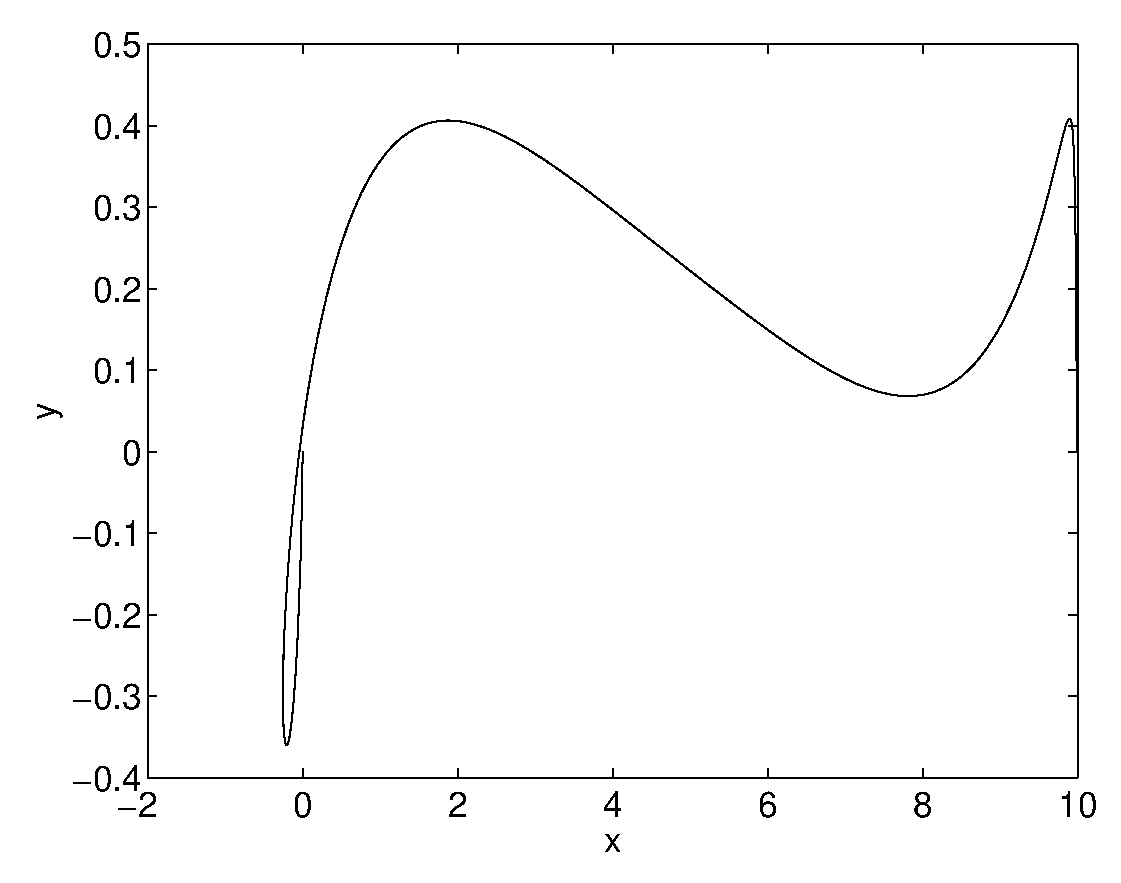
\includegraphics[height=0.3\textheight]{img/final_15_1_10_path.eps} %TODO make proper image
\caption{Error norm w.r.t iteration, discontinuous model of the platform}
\label{fig:error_discont}
\end{figure}

\section{Mobile manipulator}
This section covers the simulations for the whole RobRex mobile manipulator. Two types of problems will
be discussed here: with constraints only for the end-effector configuration and with constraints for
both mobile platform and the effector.
\subsection{Problems formulation}
The initial conditions for both tasks are: $q_0 = [w_0; \dot{w}_0] = (0, 0, a\frac{\pi}{2}, 0_7)^T$, 
$x_0 = \left(
x_1 ,\, x_2 ,\, x_4 ,\, x_5
\right) = \left(
\frac{\pi}{4} ,\, \frac{\pi}{5} ,\, \frac{\pi}{6} ,\, -\frac{\pi}{3}
\right).$ The control horizon for these tasks is $T=20\,\mathrm{s}$.
\subsubsection{Problem one}
This motion planning problem regards only the end position of the effector
and the velocities of the platform. 
The coordinates in global task space $(x, y, z, \phi, \theta, \psi) $ should be equal to
$(10, 0, 0.2, \frac{\pi}{2}, \frac{\pi}{4}, -\frac{\pi}{2})$. The velocity of each platform coordinate
should be equal to zero. Such constraints guarantee that the whole system will stand still at the end
of the motion.
\subsubsection{Problem two}
This case is related to the platform pose as well as to the configuration of the effector.
As far as the platform is concerned, the constraints are put only on the $x$ coordinate and
the velocities. The desired values are $(x_p, \dot{w}) = (10, 0, 0, 0, 0, 0)$. When it comes to
the effector, the we want the following set of coordinate in global task space: $(y, \phi, \theta, \psi)
= (0, \frac{\pi}{2}, \frac{\pi}{4}, -\frac{\pi}{2})$.

\subsection{Simulation conditions}
The platform parameter has been set as in section \ref{sec:pltf_params}. The lenghts of the links
are equal to:
\begin{multicols}{2}
\begin{itemize}
\item $a_2=0.1276 \,\mathrm{m}$,
\item $a_3=0.041 \,\mathrm{m}$,
\item $a_4=0.2615 \,\mathrm{m}$,
\item $a_5=0.0195 \,\mathrm{m}$.
\end{itemize}
\end{multicols}
First and second joint of the manipulator are actually in the same place, so we assume that $a_1=0$.

\subsection{Simulation results}
The outcome of the simulations are presented in figure \ref{fig:pr1} for the problem one and in figure
\ref{fig:pr2} for the problem two. These figures include the plots of the error with respect to the
iteration, the platform path, the slips values and the inputs. The angles computed for joints are
presented in table \ref{tab:effector}. Regarding the control inputs parameters, table \ref{tab:in_eff}
shows the total energy values of the signal and the maximum amplitudes.

\begin{figure}
\begin{subfigure}[b]{0.45\textwidth}
\centering
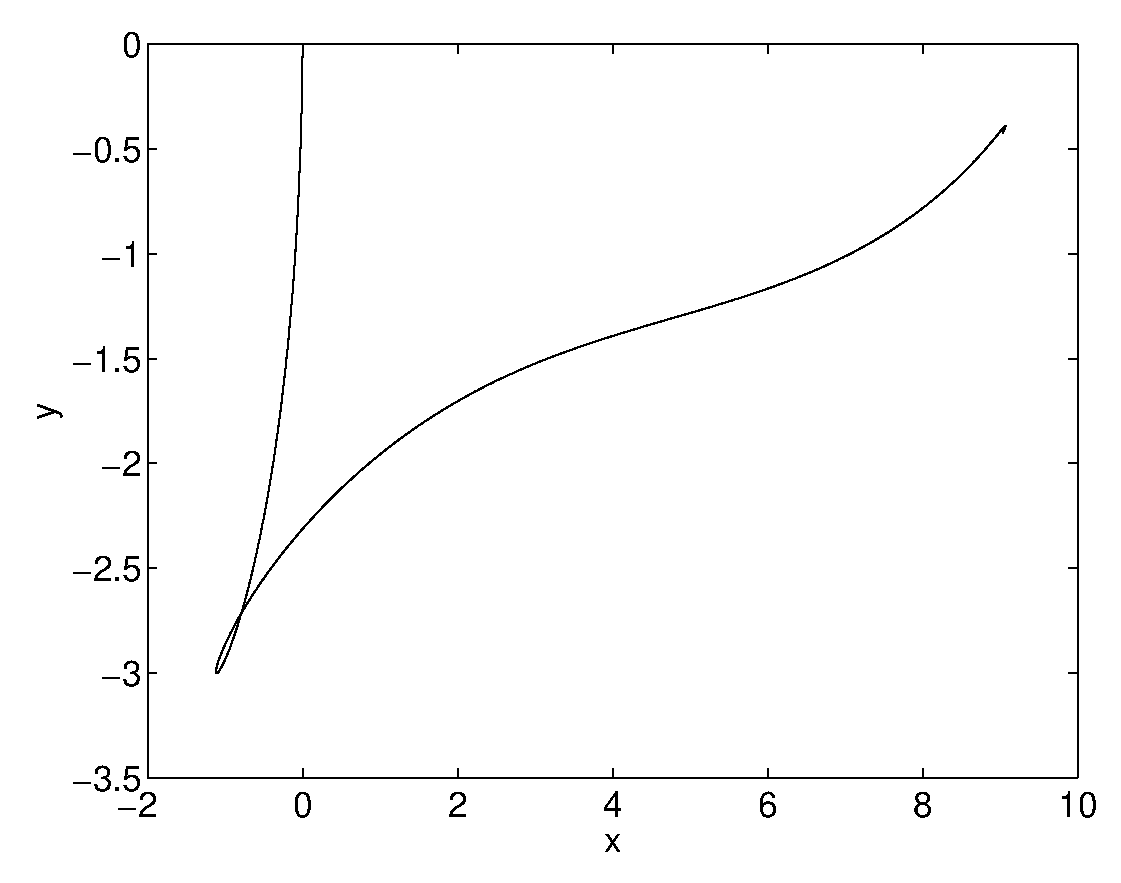
\includegraphics[width=\textwidth]{img/manip_task_path.eps}
\caption{path}
\end{subfigure}
~
\begin{subfigure}[b]{0.45\textwidth}
\centering
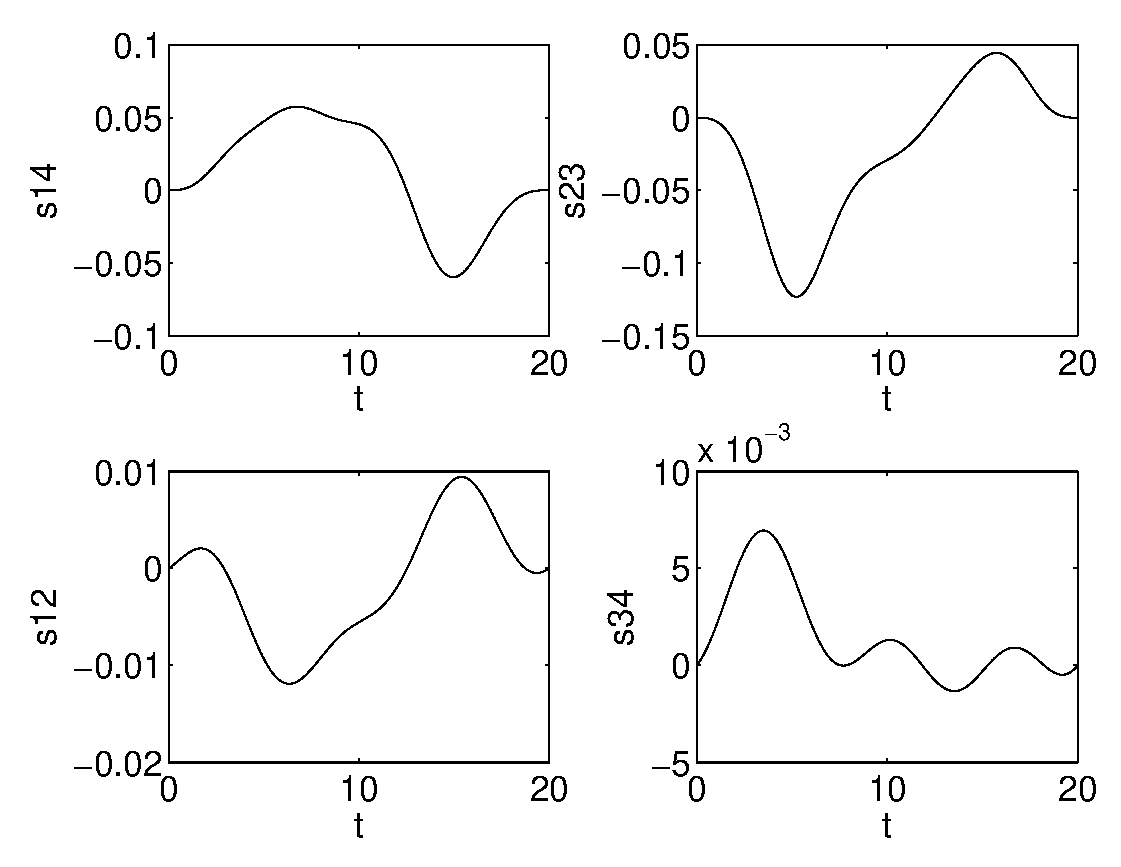
\includegraphics[width=\textwidth]{img/manip_task_slips.eps}
\caption{slips}
\end{subfigure}

\begin{subfigure}[b]{0.45\textwidth}
\centering
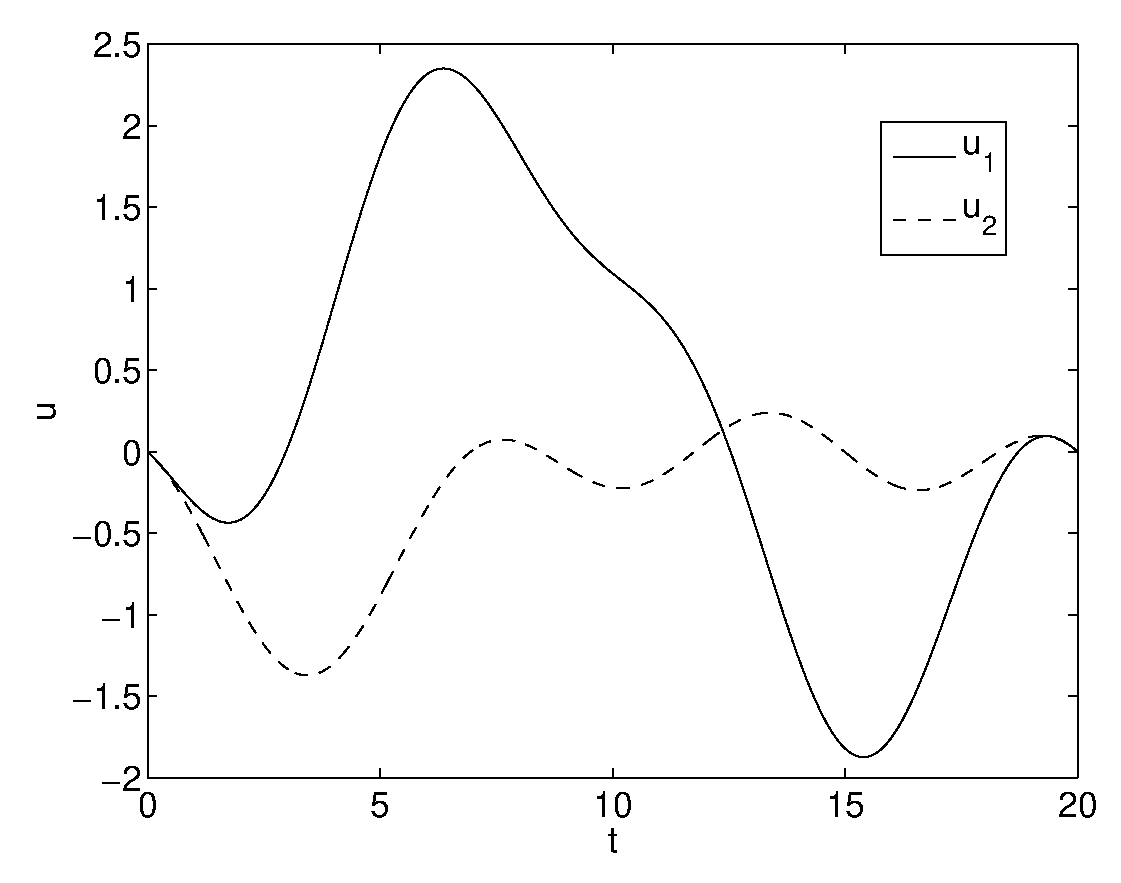
\includegraphics[width=\textwidth]{img/manip_task_u.eps}
\caption{control inputs}
\end{subfigure}
~
\begin{subfigure}[b]{0.45\textwidth}
\centering
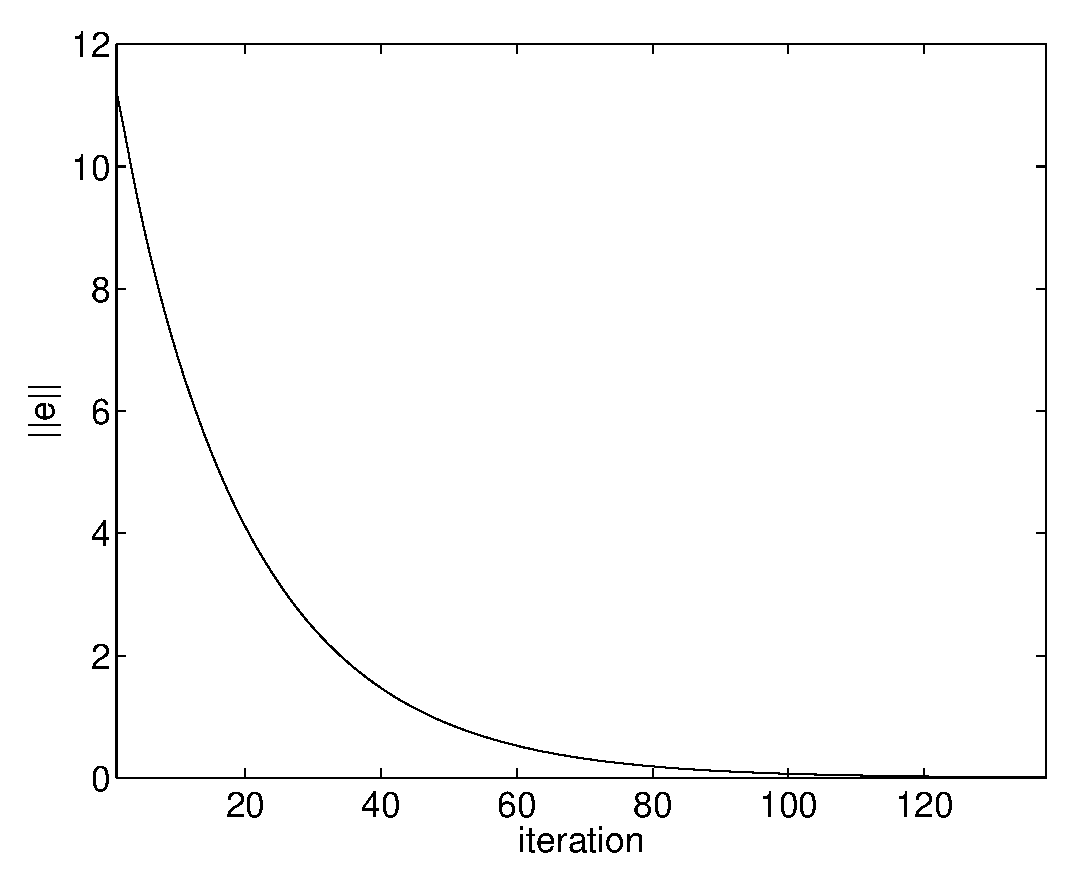
\includegraphics[width=\textwidth]{img/manip_task_err.eps}
\caption{error norm}
\end{subfigure}
\caption{Problem one}
\label{fig:pr1}
\end{figure}

\begin{figure}
\begin{subfigure}[b]{0.45\textwidth}
\centering
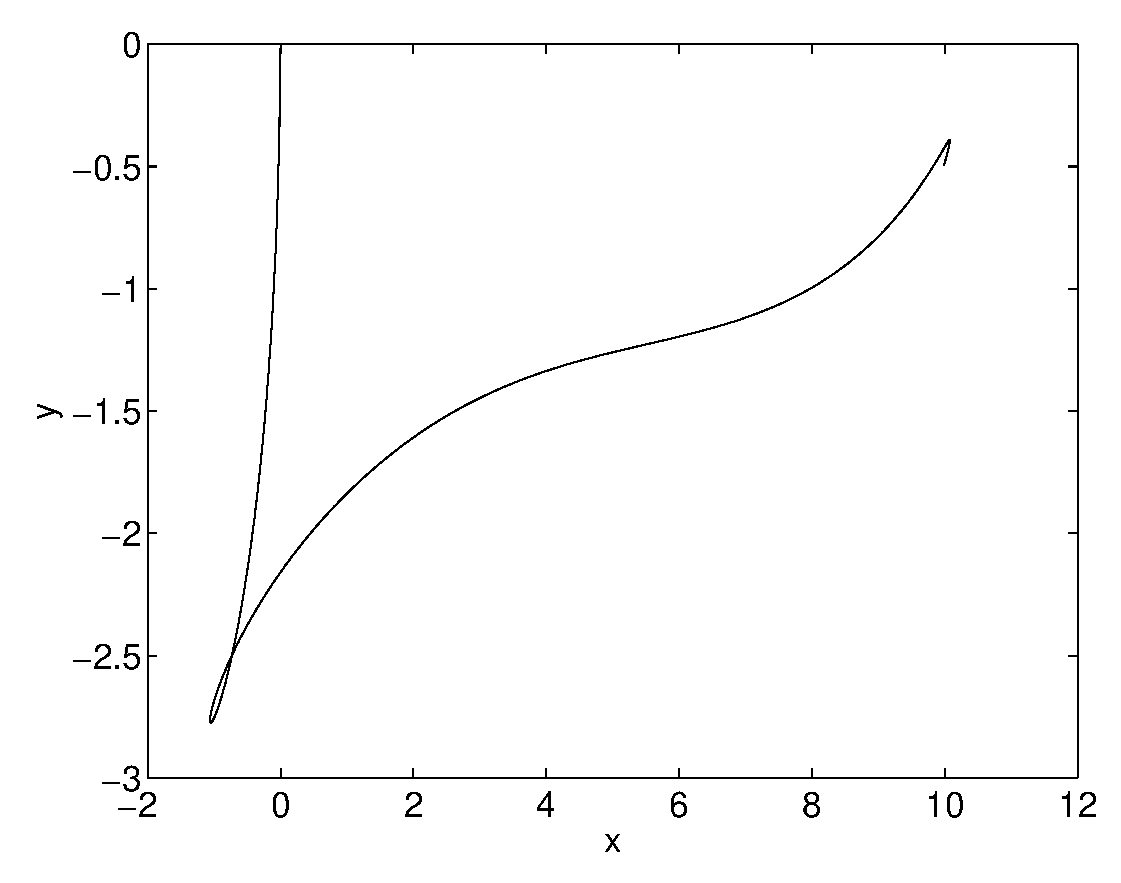
\includegraphics[width=\textwidth]{img/manip_pltf_task_path.eps}
\caption{path}
\end{subfigure}
~
\begin{subfigure}[b]{0.45\textwidth}
\centering
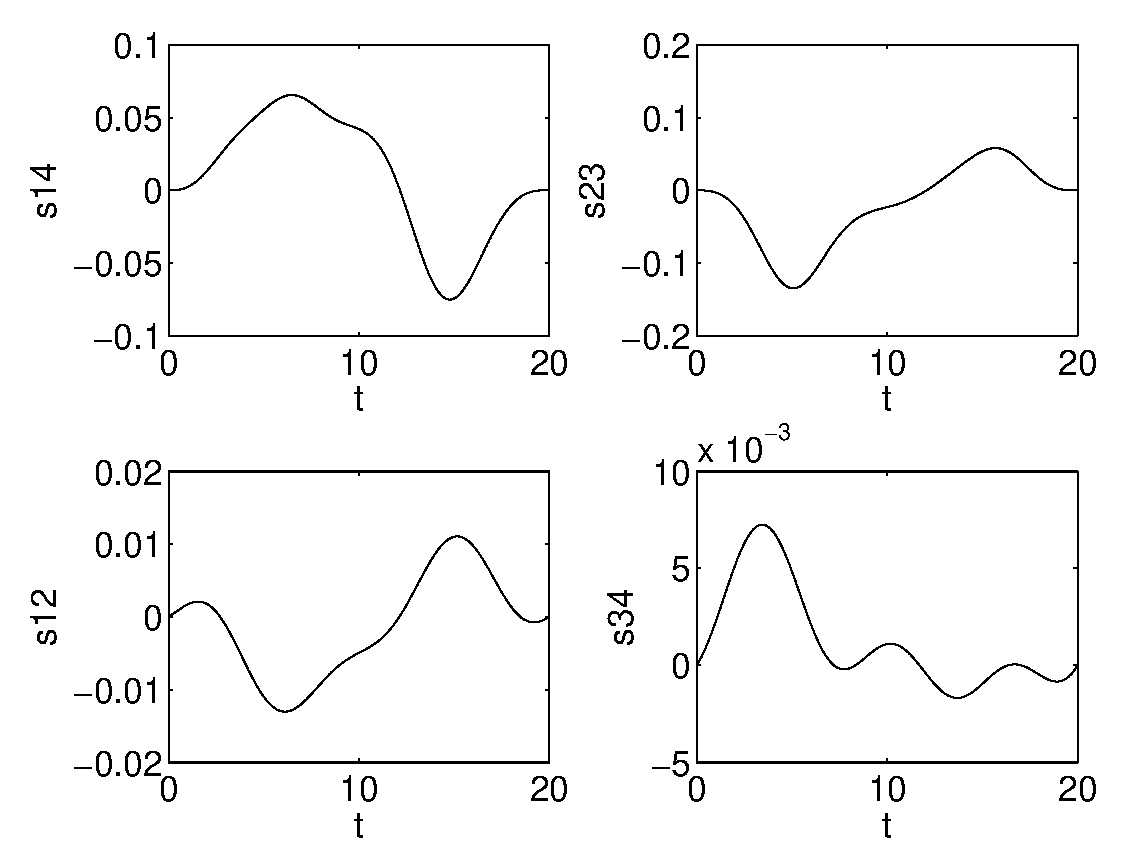
\includegraphics[width=\textwidth]{img/manip_pltf_task_slips.eps}
\caption{slips}
\end{subfigure}

\begin{subfigure}[b]{0.45\textwidth}
\centering
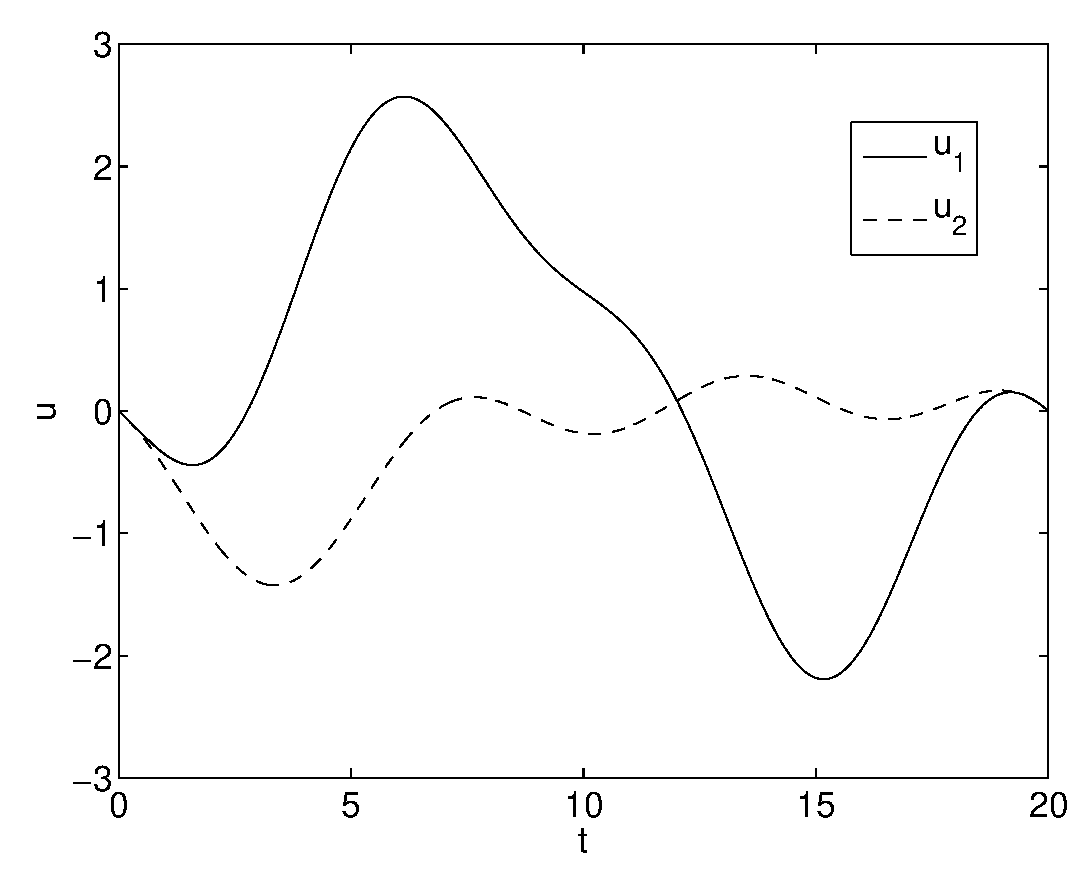
\includegraphics[width=\textwidth]{img/manip_pltf_task_u.eps}
\caption{control inputs}
\end{subfigure}
~
\begin{subfigure}[b]{0.45\textwidth}
\centering
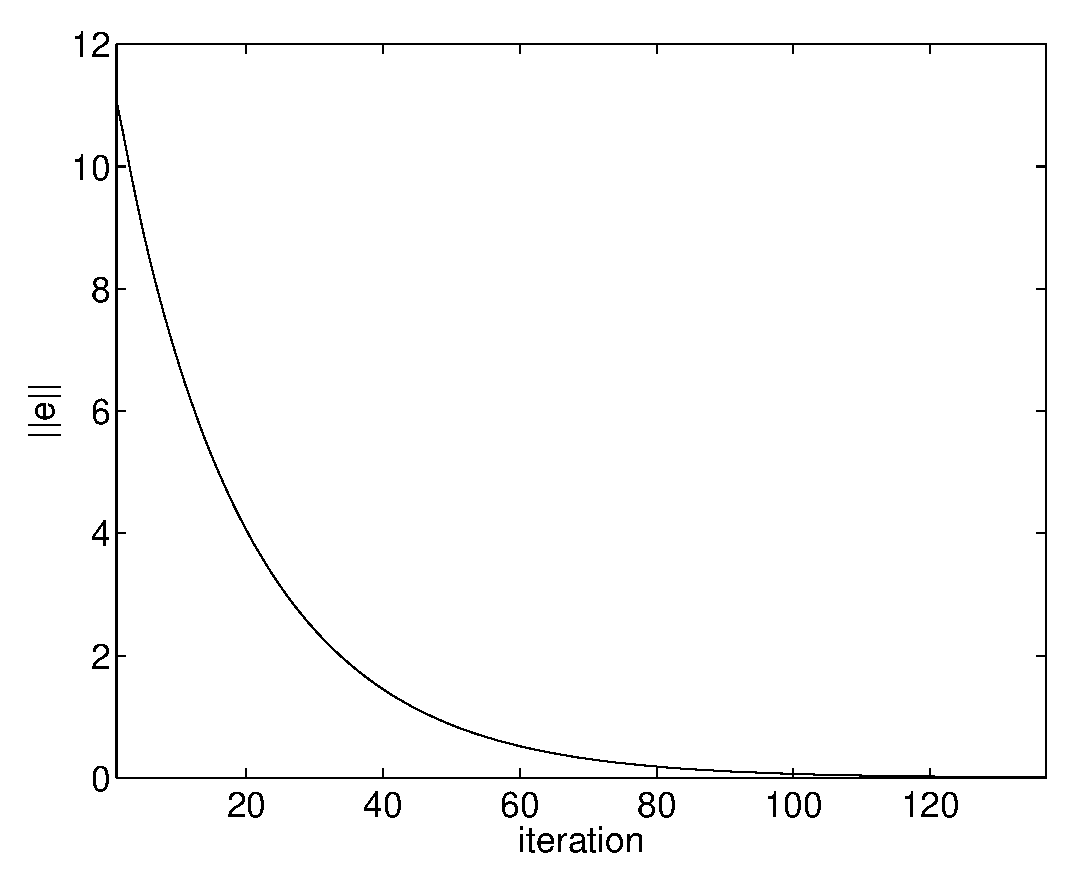
\includegraphics[width=\textwidth]{img/manip_pltf_task_err.eps}
\caption{error norm}
\end{subfigure}
\caption{Problem two}
\label{fig:pr2}
\end{figure}